\documentclass[12pt,a4paper]{article}
\usepackage[UTF8,zihao=-4]{ctex}
\usepackage[top=2.5cm,bottom=2.5cm,left=2.8cm,right=2.8cm]{geometry}
\usepackage{fontspec}
\setmainfont{Times New Roman}
\usepackage{setspace}
\setstretch{1.5}
\setlength{\parskip}{0pt}
\usepackage{graphicx,float,booktabs,array,makecell,adjustbox,amsmath,amssymb,chngcntr,caption,fancyhdr,hyperref,titlesec,subcaption}
\graphicspath{{./}{plots/}}
\counterwithin{figure}{section}
\counterwithin{table}{section}
\renewcommand{\thefigure}{\arabic{section}-\arabic{figure}}
\renewcommand{\thetable}{\arabic{section}-\arabic{table}}
\captionsetup{font=small,labelsep=space,justification=centering,aboveskip=6pt,belowskip=12pt}
\captionsetup[table]{aboveskip=12pt,belowskip=6pt,position=above}
\setlength{\headheight}{15pt}
\pagestyle{fancy}
\fancyhf{}
\fancyhead[C]{\small 实验报告}
\fancyfoot[C]{\small\thepage}
\hypersetup{colorlinks=true,linkcolor=black,citecolor=black,urlcolor=blue,bookmarks=true,bookmarksnumbered=true}
\titleformat{\section}[block]{\centering\heiti\zihao{4}}{\thesection}{1em}{}
\titlespacing*{\section}{0pt}{24pt}{18pt}
\titleformat{\subsection}[hang]{\heiti\zihao{-4}}{\thesubsection}{1em}{}
\titlespacing*{\subsection}{0pt}{18pt}{6pt}
\newcommand{\IzeroValue}{10.04\,\mathrm{mW}}

\begin{document}
\begin{titlepage}
  \centering
  \vspace*{3cm}
  {\heiti\zihao{2} 实验报告}\\[1cm]
  {\heiti\zihao{3} 偏振与波片认识}\\[2cm]
  \begin{tabular}{ll}
    姓\quad 名： & 叶哲昊 \\[0.5cm]
    学\quad 号： & 24012561 \\[0.5cm]
    班\quad 级： & \underline{\hspace{6cm}} \\[0.5cm]
    实验日期： & 2024年5月8日 \\
  \end{tabular}
  \vfill
\end{titlepage}

\tableofcontents
\newpage
\setcounter{page}{1}

\section{实验目的}
本实验围绕线偏振光、椭圆偏振光与圆偏振光的产生和判别展开，目标是：理解起偏器与检偏器的工作机理，掌握用光功率计测量透射光强并绘制偏振特征曲线的方法；在真实实验数据基础上验证 $1/4$ 波片对偏振态的调制作用，说明其在入射偏振方向与波片光轴夹角分别为 $0^{\circ}$、$30^{\circ}$ 和 $45^{\circ}$ 时，对应线偏振、椭圆偏振和近似圆偏振的实验结果；验证 $1/2$ 波片能够在保持线偏振属性的同时使振动方向旋转 $2\alpha$，并通过曲线峰位的移动量给出定量判据。

\section{实验原理}
光是横波，其电矢量始终垂直于传播方向。若电矢量方向保持不变，仅大小随时间变化，则光为线偏振光；若电矢量大小不变而方向匀速转动，则为圆偏振光；若大小和方向都随时间有规律变化，则为椭圆偏振光。将光矢量分解到互相正交的两个方向，可写成
\begin{equation}
E_x=a_1\cos\omega t,\qquad E_y=a_2\cos(\omega t+\delta).
\end{equation}
消去时间参量后得到偏振椭圆方程
\begin{equation}
\frac{E_x^2}{a_1^2}+\frac{E_y^2}{a_2^2}-2\frac{E_xE_y}{a_1a_2}\cos\delta=\sin^2\delta.
\end{equation}
当 $\delta=0$ 或 $\pi$ 时，轨迹退化为直线；当 $\delta=\pm\pi/2$ 且 $a_1=a_2$ 时，轨迹为圆，这正是圆偏振光的判据。

起偏器用于获得方向确定的线偏振光，检偏器则用于分析透射光的偏振状态。对于线偏振光，若检偏器透振方向与入射振动方向夹角为 $\theta$，则光强满足马吕斯定律
\begin{equation}
I=I_0\cos^2\theta.
\end{equation}
因此，线偏振光经过检偏器后应表现为可消光的 $\cos^2\theta$ 变化规律。

波片由双折射晶体制成，入射线偏振光可分解为沿快轴和慢轴振动的两个分量。设波片厚度为 $d$，普通光与非普通光折射率分别为 $n_o$ 和 $n_e$，则光程差与相位差为
\begin{equation}
\Delta=|n_o-n_e|d,\qquad \delta=\frac{2\pi}{\lambda}|n_o-n_e|d.
\end{equation}
当波片为 $1/4$ 波片时，$\delta\approx\pi/2$。若入射线偏振光与波片光轴夹角为 $0^{\circ}$，出射仍为线偏振光；夹角为 $30^{\circ}$ 时，两正交分量振幅不等且相差 $\pi/2$，得到椭圆偏振光；夹角为 $45^{\circ}$ 时，两分量等幅并相差 $\pi/2$，得到圆偏振光。对于 $1/2$ 波片，$\delta\approx\pi$，出射光仍保持线偏振，但振动方向相对快轴旋转 $2\alpha$。因此，检偏器扫描曲线应整体发生相位平移，而波形仍保持近似 $\cos^2$ 规律。

据此，本实验的判据十分直接：若旋转检偏器时光强能够完全消光，则出射光为线偏振光；若光强有起伏但无法消光，则为椭圆偏振光；若光强近似恒定，则为圆偏振光或近似圆偏振光。结合极坐标图和 $I/I_0$ 与 $\cos^2\theta$ 的关系图，可以进一步判断波片对偏振态的调制效果。

\section{实验仪器}
实验所用仪器包括激光器、圆形可调衰减片、起偏器 $P$、检偏器 $A$、$1/4$ 波片、$1/2$ 波片、光功率计以及光学平台与光具座。实验中先由起偏器产生稳定的线偏振光，再在 $P$ 与 $A$ 之间插入不同波片，通过功率计逐点记录透射光强。图\ref{fig:setup-photo} 给出了实验时的实际光路布置，图\ref{fig:platform-photo} 展示了整理器材后的平台整体状态。

\begin{figure}[H]
  \centering
  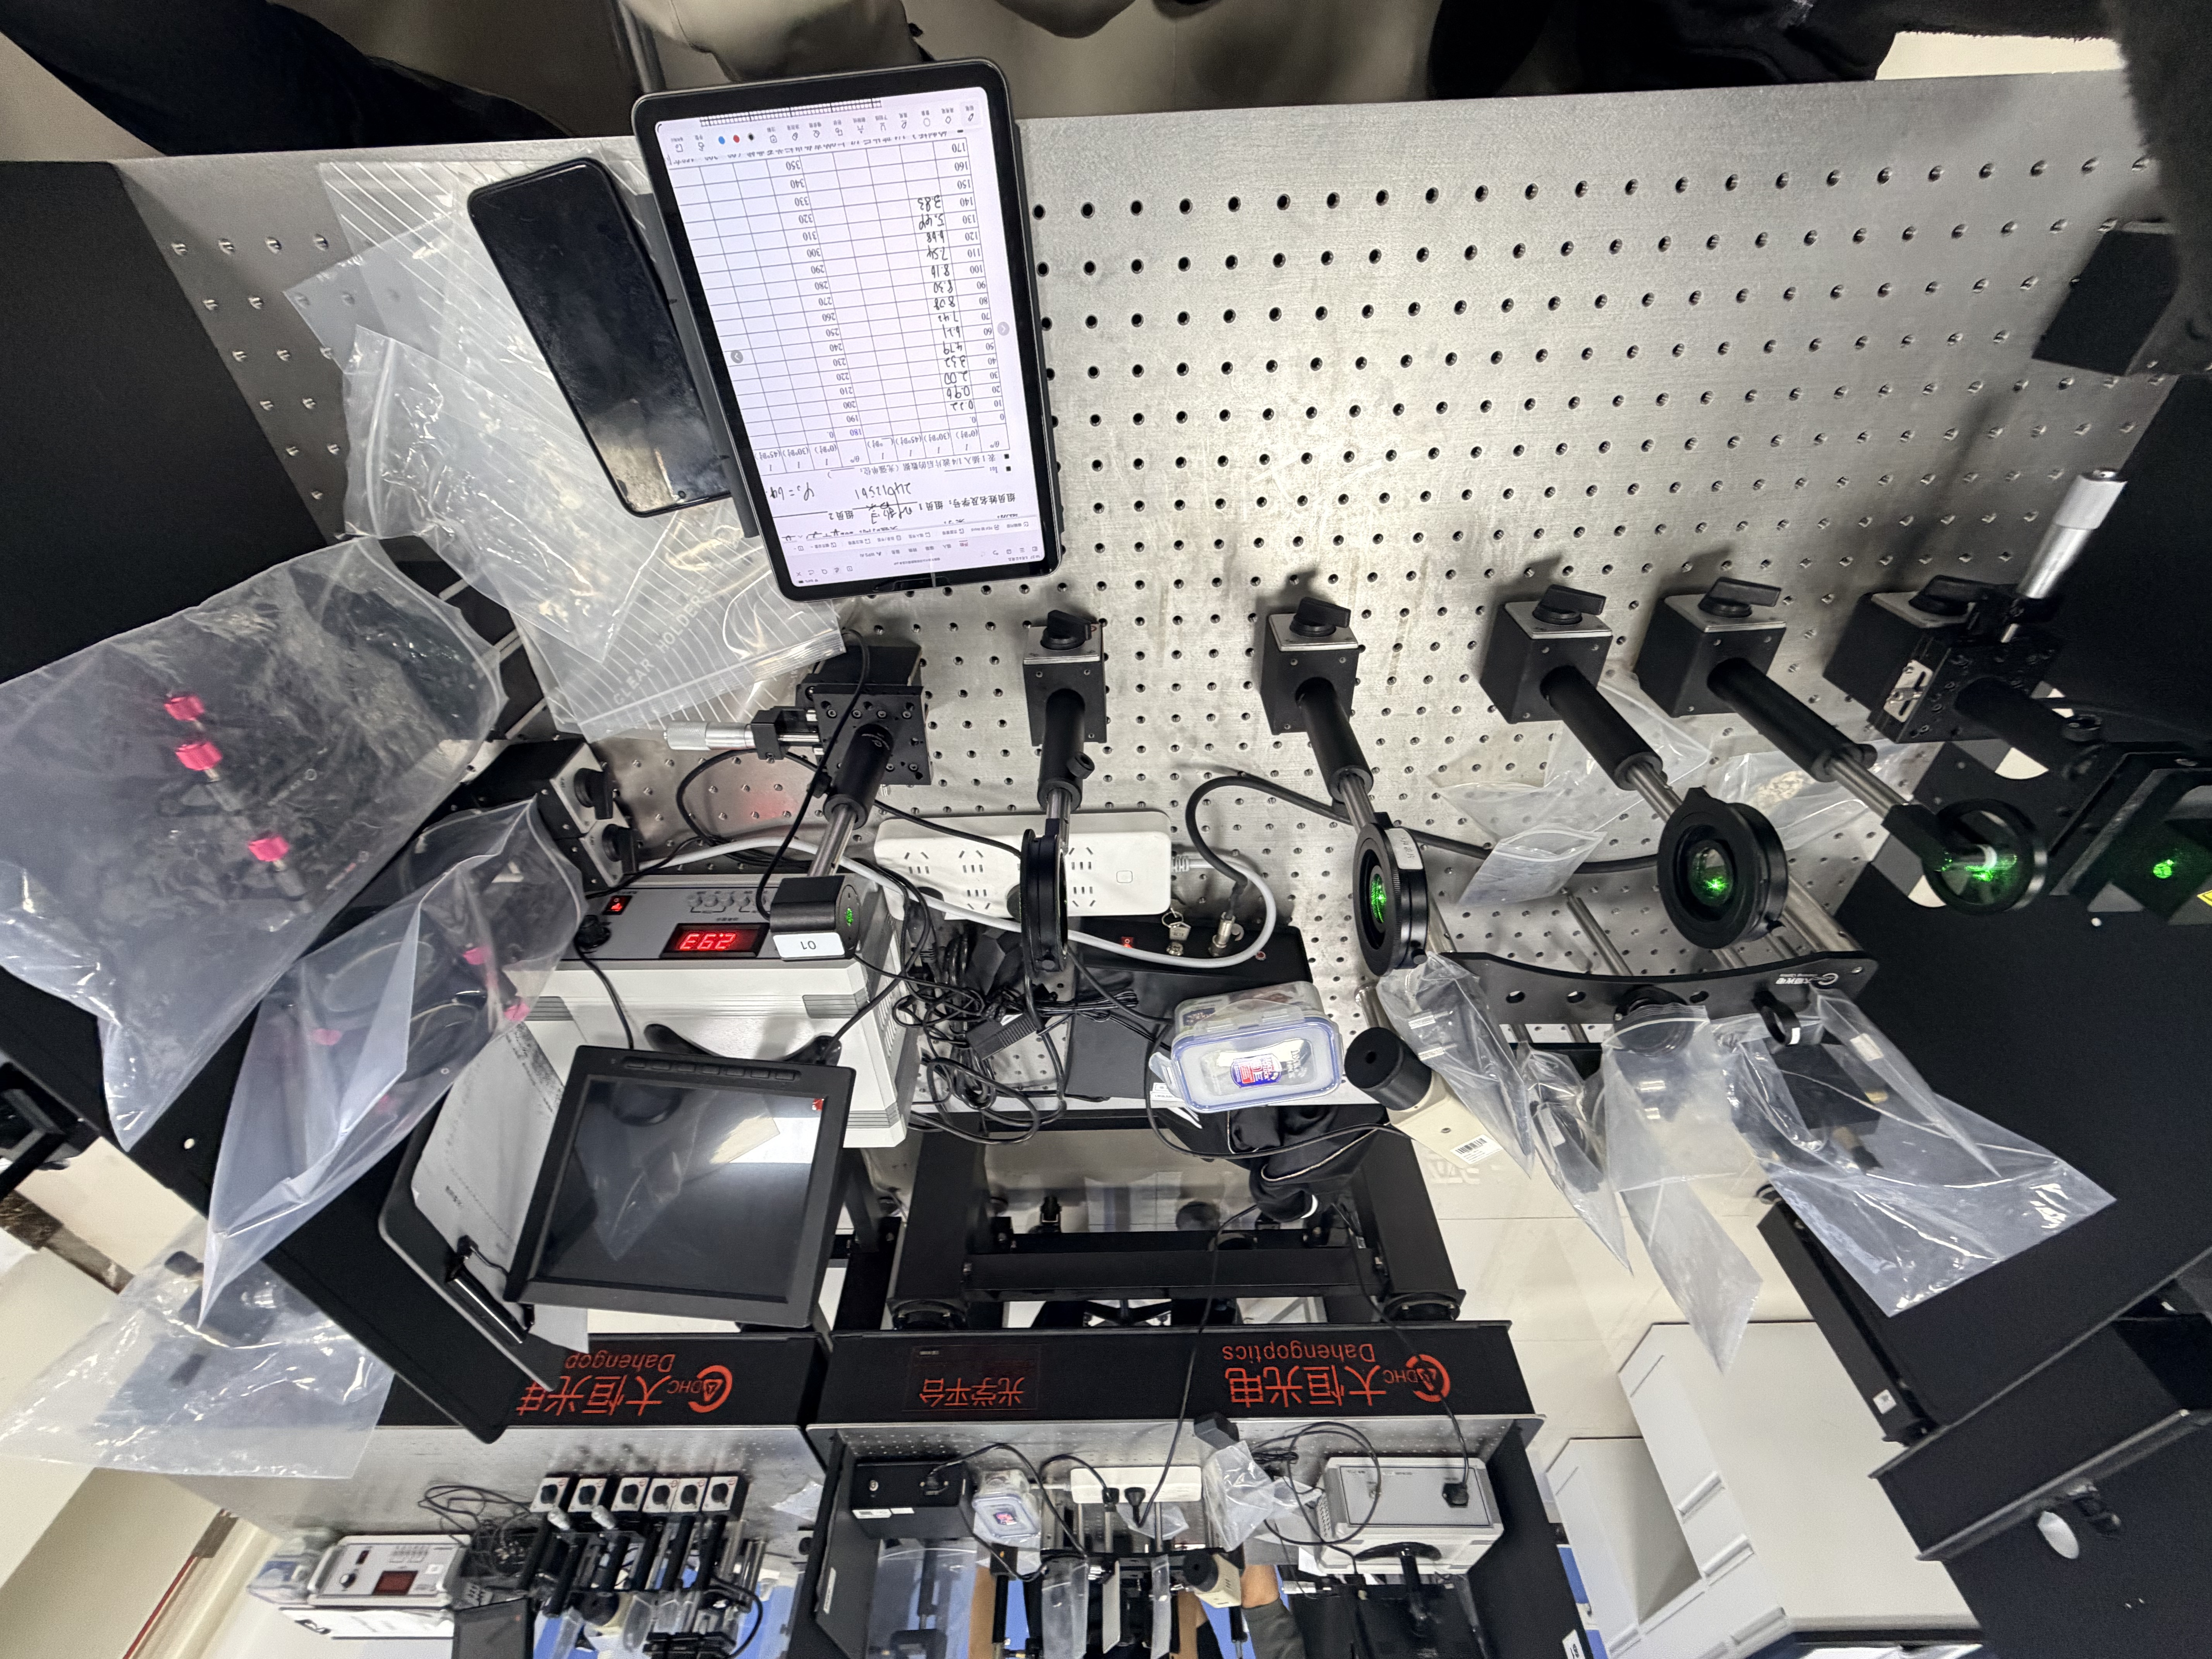
\includegraphics[width=0.84\textwidth]{实验光路照片.jpg}
  \caption{偏振与波片认识实验光路实拍图}
  \label{fig:setup-photo}
\end{figure}

\begin{figure}[H]
  \centering
  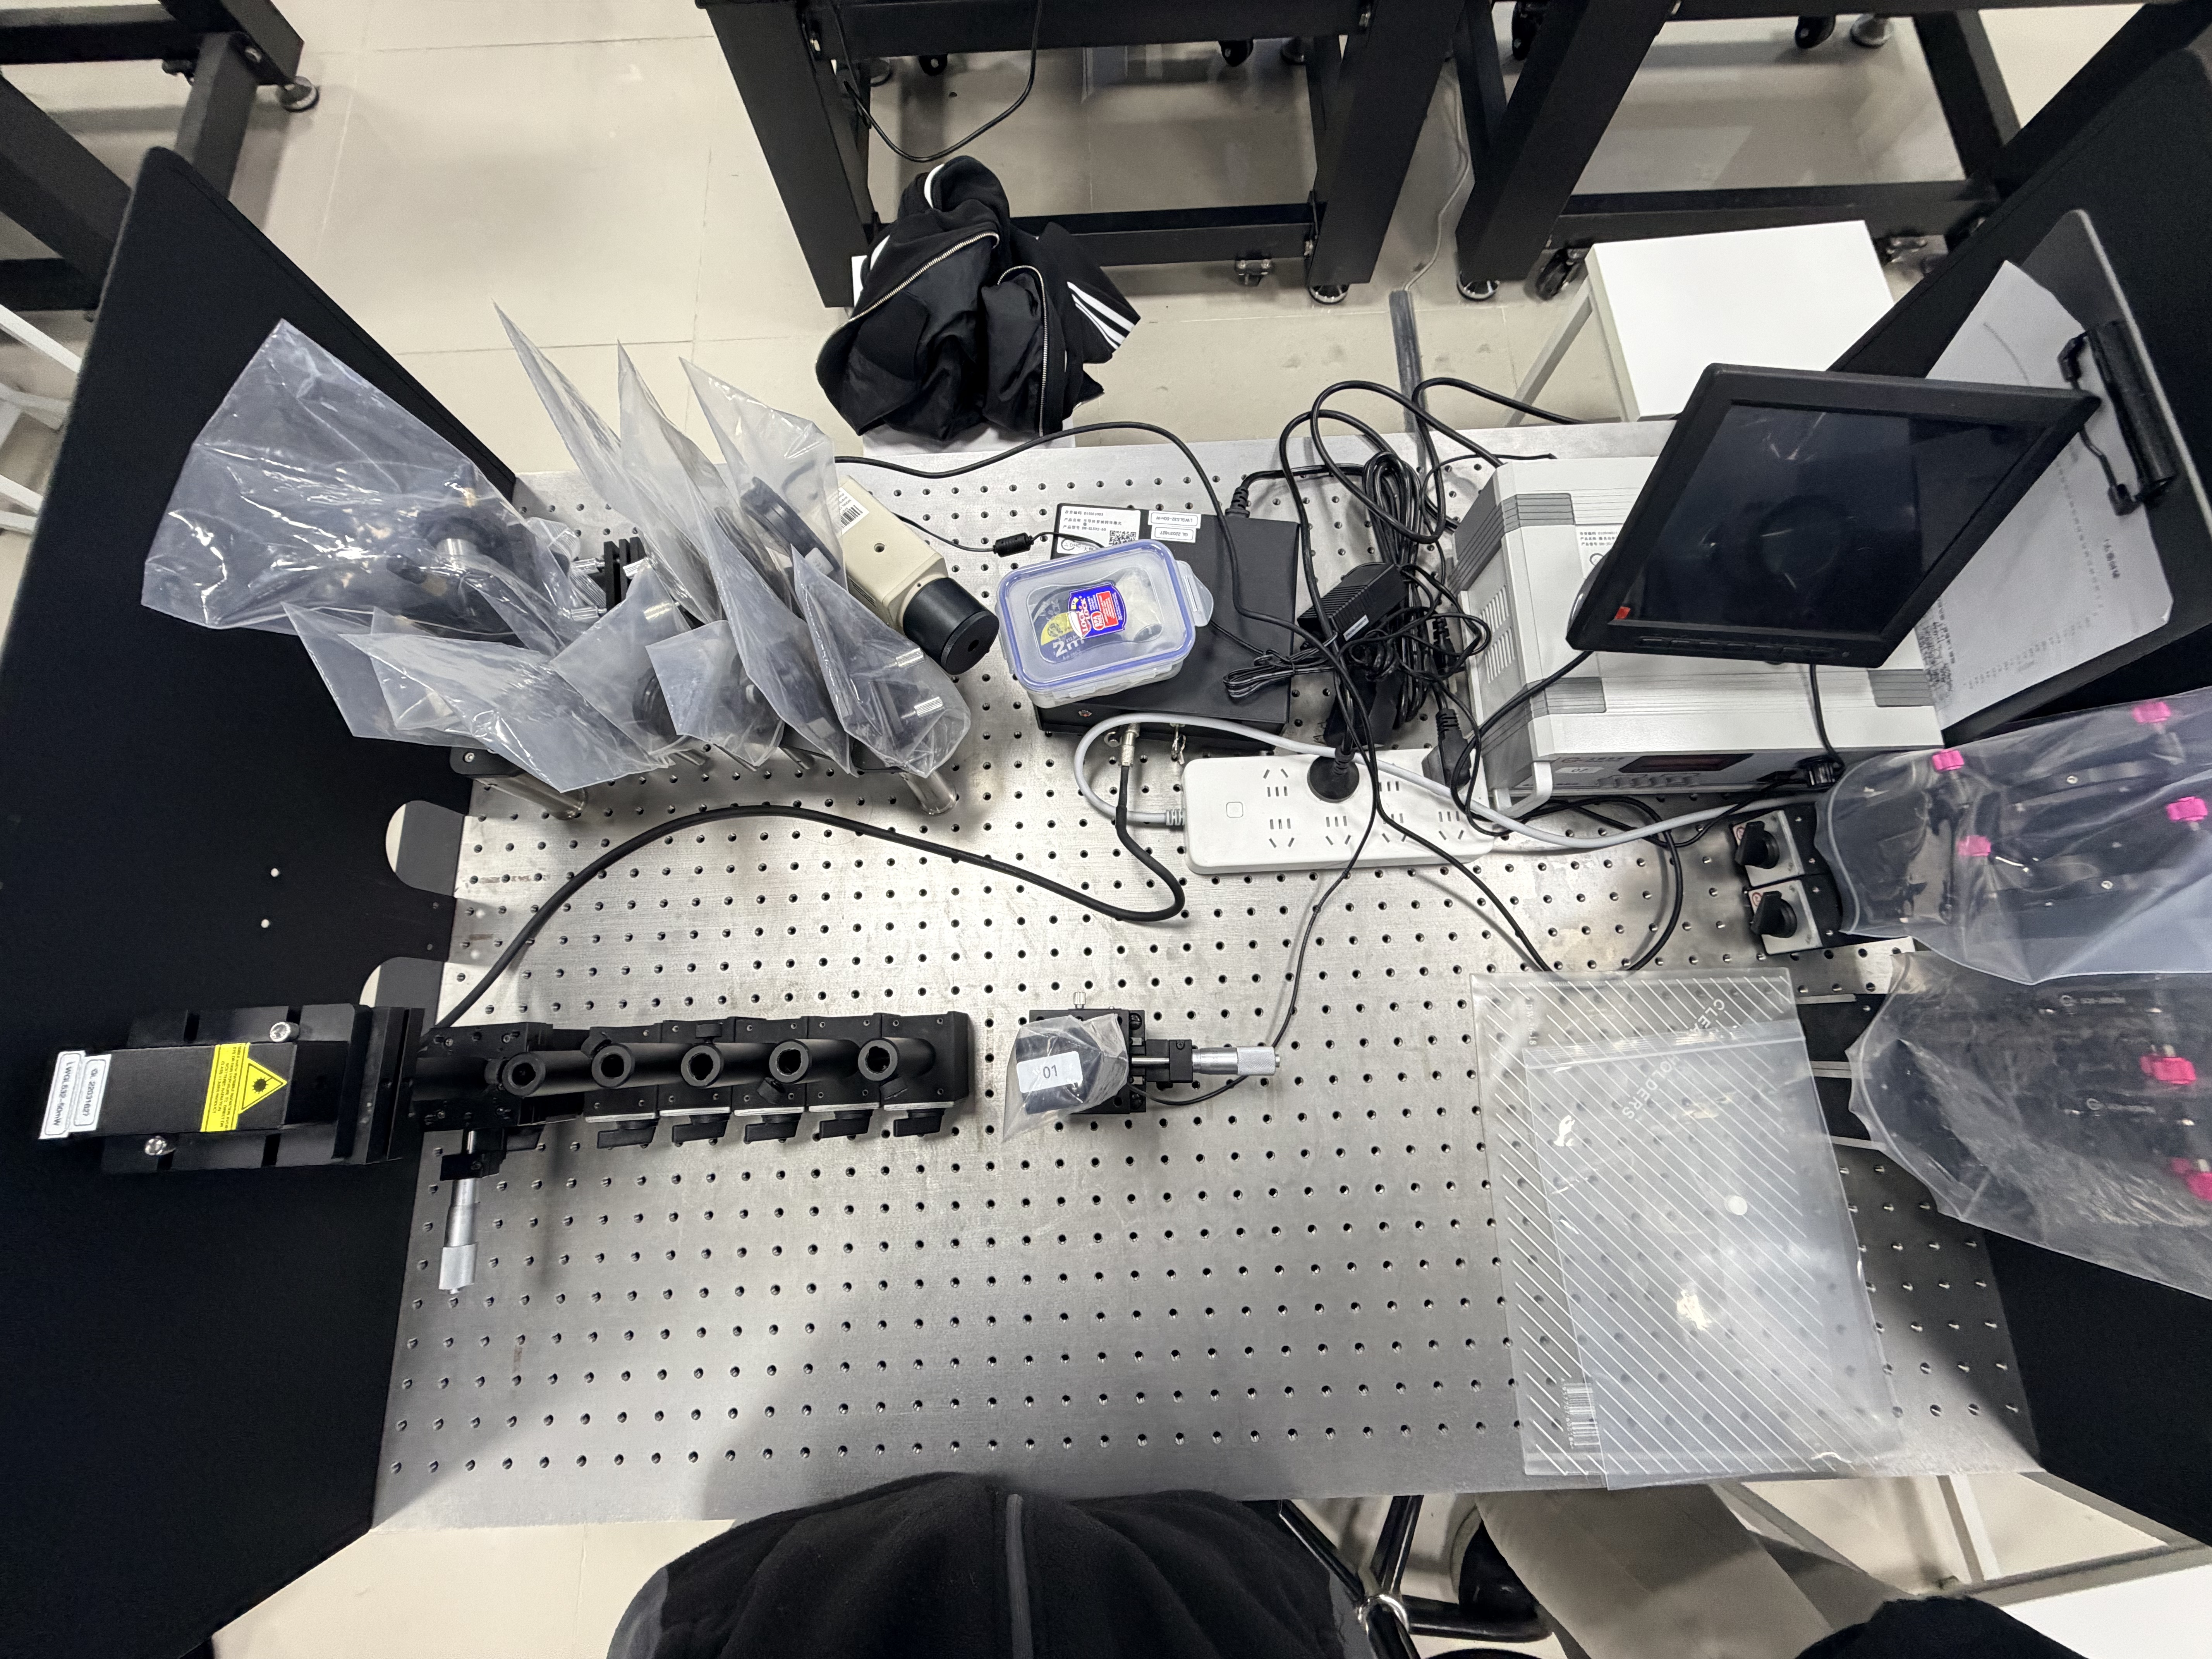
\includegraphics[width=0.78\textwidth]{完成器材整理后的照片.jpg}
  \caption{实验结束后器材整理状态}
  \label{fig:platform-photo}
\end{figure}

\section{实验步骤}
实验首先搭建基础光路，使激光器、衰减片、起偏器、检偏器和功率计严格共轴，并将功率计量程预置在 $20\,\mathrm{mW}$ 档。移去检偏器后旋转起偏器，使功率计示数达到最大并记录起偏器角度盘读数 $\theta_0=286^{\circ}$；随后安装检偏器并旋转至系统消光，记录此时读数 $\theta_1=317.5^{\circ}$，作为后续所有测量的参考零位。

在验证 $1/4$ 波片作用时，保持检偏器位于消光位置，在 $P$ 与 $A$ 之间插入 $1/4$ 波片并旋转直至系统重新消光，记录波片零位 $\varphi_0=64.5^{\circ}$。以该位置对应的相对夹角定义为 $\theta=0^{\circ}$，再分别将波片转到 $0^{\circ}$、$30^{\circ}$、$45^{\circ}$ 和补充测量的 $75^{\circ}$ 位置。每到一个位置后，都让检偏器从参考零位开始每隔 $10^{\circ}$ 扫描一次，并记录一周内的透射光强。

在验证 $1/2$ 波片作用时，将 $1/4$ 波片取下，插入 $1/2$ 波片并同样通过重新消光的方法标定零位，得到 $\varphi_0'=115.5^{\circ}$。之后按与前一部分完全相同的扫描方式记录 $0^{\circ}$、$30^{\circ}$、$45^{\circ}$ 和补充测量的 $75^{\circ}$ 数据。由于记录单中的绘图区尚未手工补画，本报告采用 Python 脚本基于原始数据生成直角坐标图、极坐标图以及 $I/I_0$ 与 $\cos^2\theta$ 的关系图，用于后续分析。

\section{实验数据与处理}
原始记录单中 $I_0$ 一栏未单独填入数值，因此本报告在作图归一化时取全部测量中的最大光强 $10.04\,\mathrm{mW}$ 作为参考值，即 $I_0=\IzeroValue$。这样既能保证所有归一化数据不超过 $1$，又便于比较不同波片角度下透射光强曲线的形状差异。原始数据均由记录单逐项转录为 LaTeX 表格，并保留补充测量的 $75^{\circ}$ 数据列。

\subsection{$1/4$ 波片实验数据}
\begin{table}[H]
  \centering
  \caption{$1/4$ 波片实验数据（$0^{\circ}$ 至 $170^{\circ}$）}
  \input{generated/quarter_table_a.tex}
\end{table}

\begin{table}[H]
  \centering
  \caption{$1/4$ 波片实验数据（$180^{\circ}$ 至 $350^{\circ}$）}
  \input{generated/quarter_table_b.tex}
\end{table}

\begin{figure}[H]
  \centering
  \begin{subfigure}[b]{0.48\textwidth}\centering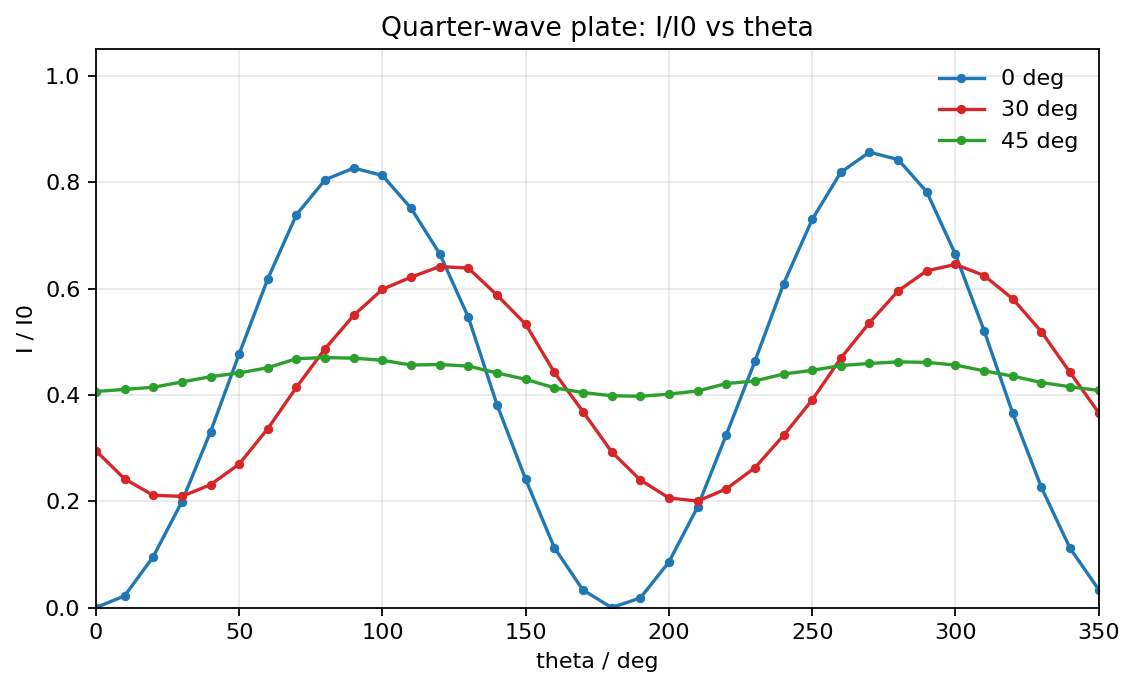
\includegraphics[width=\textwidth]{plots/quarter_cartesian.png}\caption{$I/I_0$ 与 $\theta$ 直角坐标图}\end{subfigure}\hfill
  \begin{subfigure}[b]{0.48\textwidth}\centering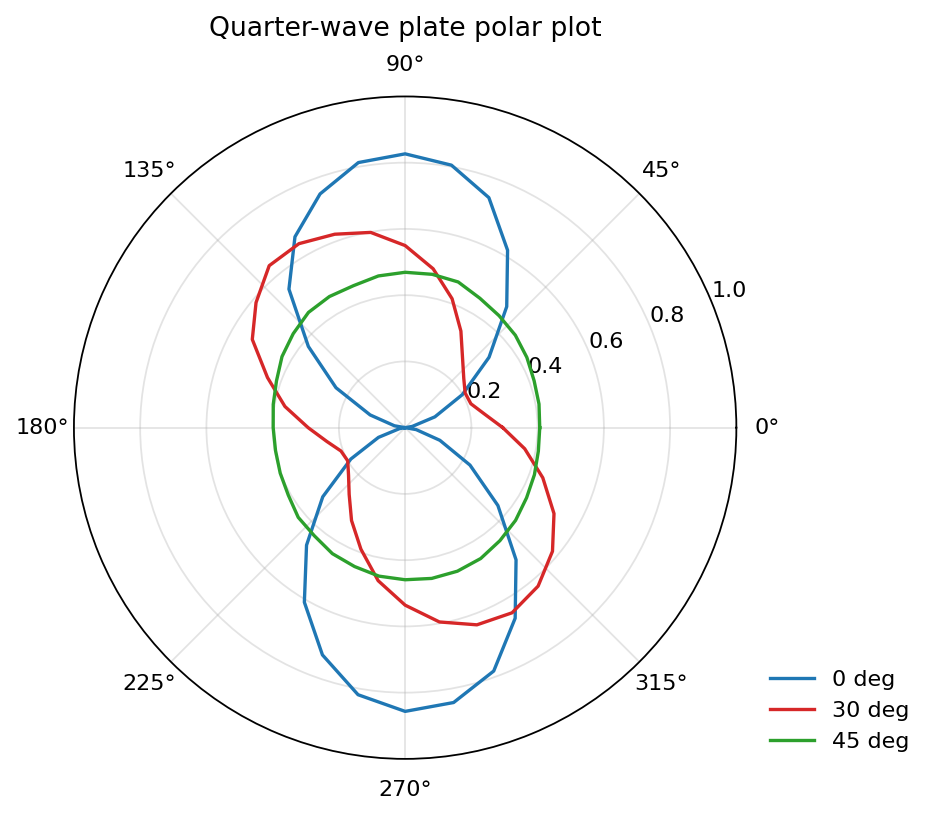
\includegraphics[width=\textwidth]{plots/quarter_polar.png}\caption{$I/I_0$ 与 $\theta$ 极坐标图}\end{subfigure}
  \caption{$1/4$ 波片作用下三组主实验数据的整体曲线}
  \label{fig:quarter-main}
\end{figure}

\begin{figure}[H]
  \centering
  \begin{subfigure}[b]{0.32\textwidth}\centering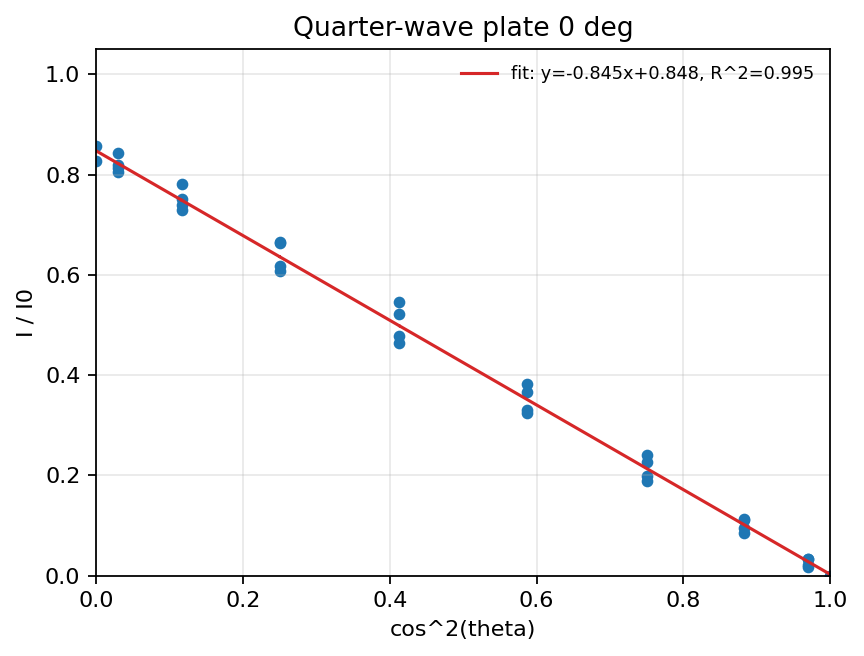
\includegraphics[width=\textwidth]{plots/quarter_cos2_0.png}\caption{$0^{\circ}$}\end{subfigure}\hfill
  \begin{subfigure}[b]{0.32\textwidth}\centering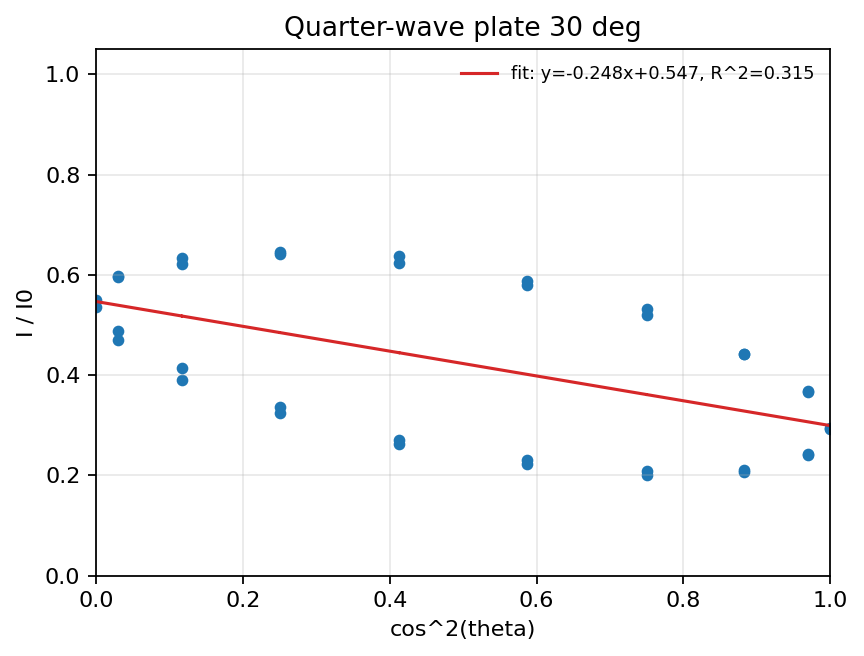
\includegraphics[width=\textwidth]{plots/quarter_cos2_30.png}\caption{$30^{\circ}$}\end{subfigure}\hfill
  \begin{subfigure}[b]{0.32\textwidth}\centering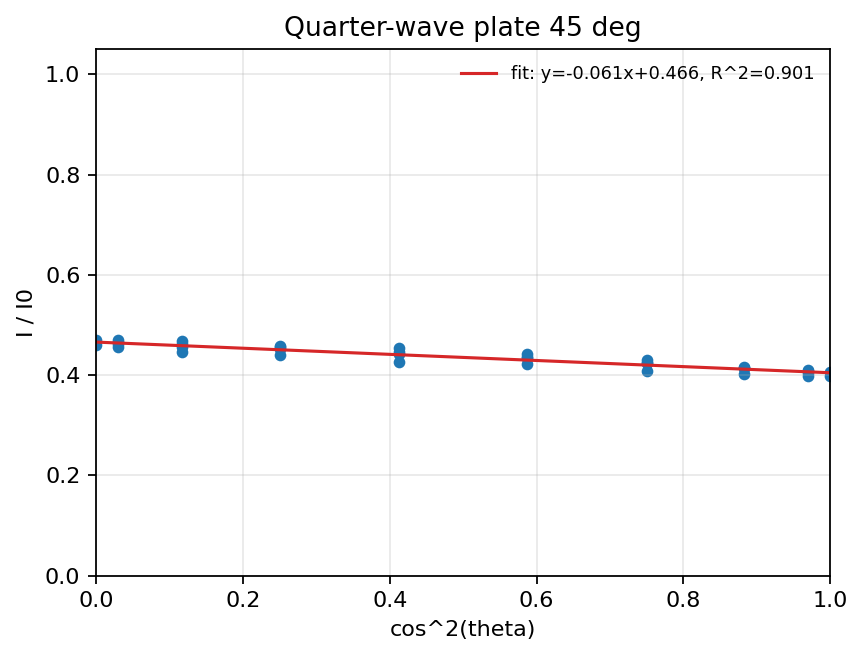
\includegraphics[width=\textwidth]{plots/quarter_cos2_45.png}\caption{$45^{\circ}$}\end{subfigure}
  \caption{$1/4$ 波片下 $I/I_0$ 与 $\cos^2\theta$ 的关系图}
  \label{fig:quarter-cos2}
\end{figure}

\subsection{$1/2$ 波片实验数据}
\begin{table}[H]
  \centering
  \caption{$1/2$ 波片实验数据（$0^{\circ}$ 至 $170^{\circ}$）}
  \begin{tabular}{ccccc}
  \toprule
  $\theta/^{\circ}$ & $I(0^{\circ})$/mW & $I(30^{\circ})$/mW & $I(45^{\circ})$/mW & $I(75^{\circ})$/mW \\
  \midrule
  0 & 0.00 & 7.19 & 10.03 & 2.58 \\
  10 & 0.38 & 5.54 & 9.76 & 4.22 \\
  20 & 1.25 & 3.82 & 8.71 & 5.91 \\
  30 & 2.56 & 2.26 & 7.45 & 7.56 \\
  40 & 4.18 & 0.97 & 5.71 & 8.88 \\
  50 & 5.99 & 0.23 & 3.90 & 9.58 \\
  60 & 7.52 & 0.04 & 2.31 & 9.78 \\
  70 & 9.01 & 0.44 & 1.08 & 9.58 \\
  80 & 9.71 & 1.39 & 0.29 & 8.58 \\
  90 & 9.85 & 2.67 & 0.04 & 7.22 \\
  100 & 9.45 & 4.22 & 0.33 & 5.70 \\
  110 & 8.52 & 5.81 & 1.17 & 3.94 \\
  120 & 7.34 & 7.59 & 2.49 & 2.50 \\
  130 & 5.87 & 8.96 & 4.17 & 1.13 \\
  140 & 4.07 & 9.81 & 5.89 & 0.25 \\
  150 & 2.38 & 10.04 & 7.49 & 0.01 \\
  160 & 1.05 & 9.56 & 8.71 & 0.34 \\
  170 & 0.24 & 8.53 & 9.55 & 1.18 \\
  \bottomrule
\end{tabular}
\end{table}

\begin{table}[H]
  \centering
  \caption{$1/2$ 波片实验数据（$180^{\circ}$ 至 $360^{\circ}$）}
  \input{generated/half_table_b.tex}
\end{table}

\begin{figure}[H]
  \centering
  \begin{subfigure}[b]{0.48\textwidth}\centering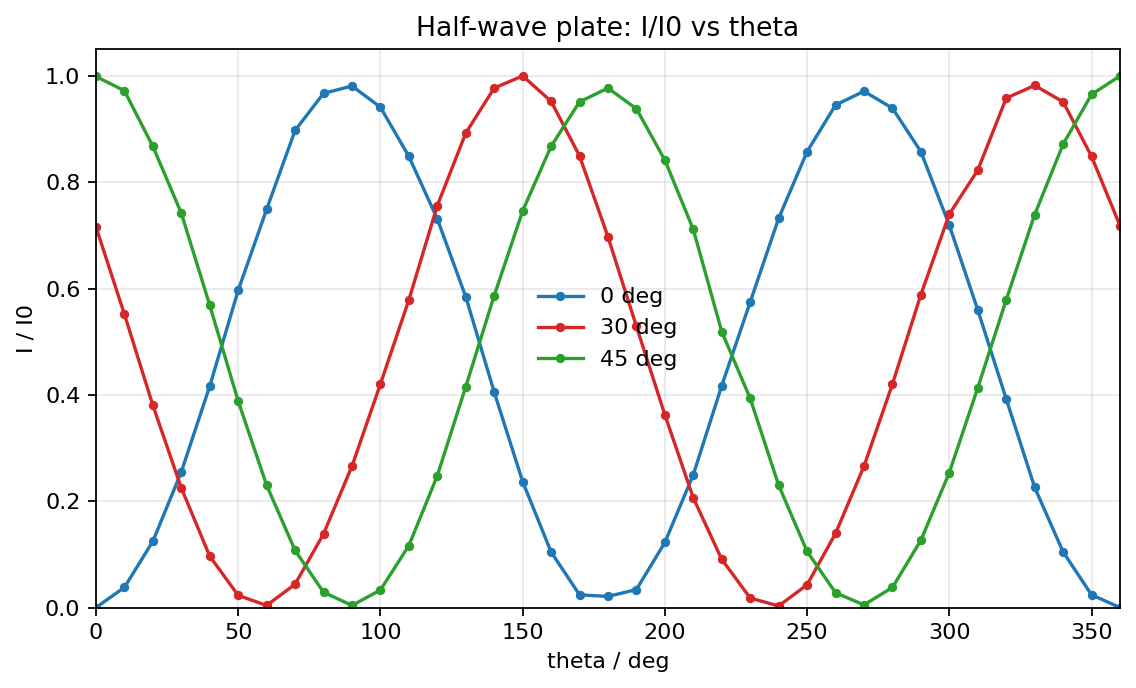
\includegraphics[width=\textwidth]{plots/half_cartesian.png}\caption{$I/I_0$ 与 $\theta$ 直角坐标图}\end{subfigure}\hfill
  \begin{subfigure}[b]{0.48\textwidth}\centering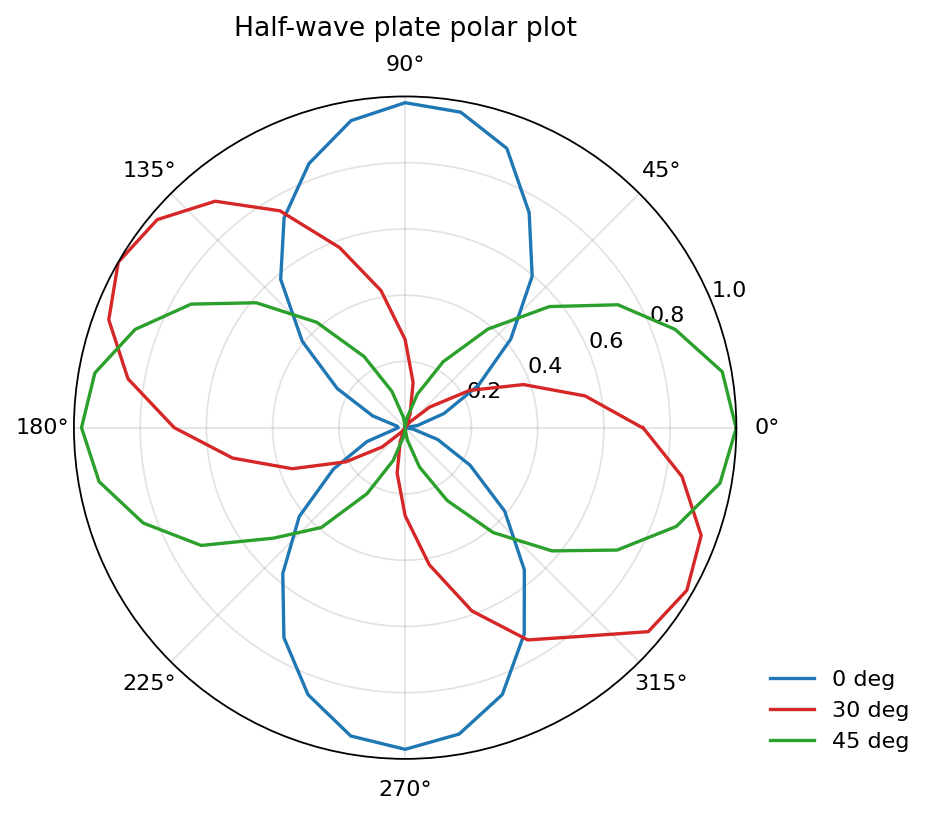
\includegraphics[width=\textwidth]{plots/half_polar.png}\caption{$I/I_0$ 与 $\theta$ 极坐标图}\end{subfigure}
  \caption{$1/2$ 波片作用下三组主实验数据的整体曲线}
  \label{fig:half-main}
\end{figure}

\begin{figure}[H]
  \centering
  \begin{subfigure}[b]{0.32\textwidth}\centering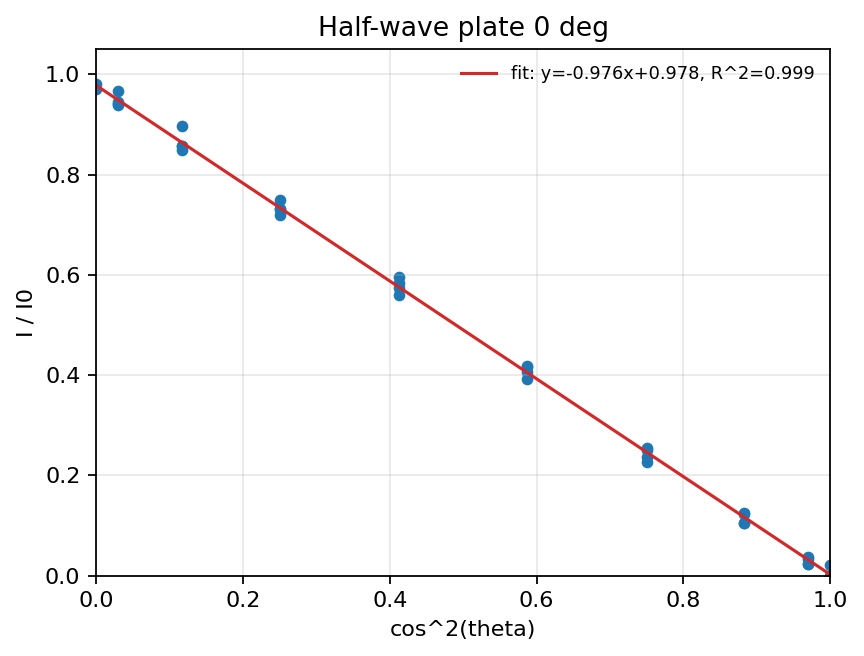
\includegraphics[width=\textwidth]{plots/half_cos2_0.png}\caption{$0^{\circ}$}\end{subfigure}\hfill
  \begin{subfigure}[b]{0.32\textwidth}\centering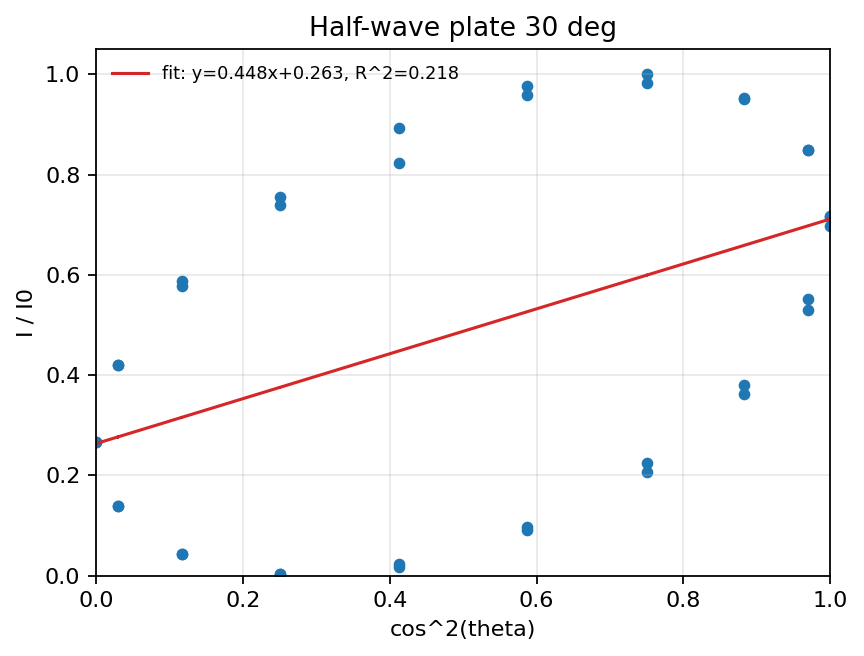
\includegraphics[width=\textwidth]{plots/half_cos2_30.png}\caption{$30^{\circ}$}\end{subfigure}\hfill
  \begin{subfigure}[b]{0.32\textwidth}\centering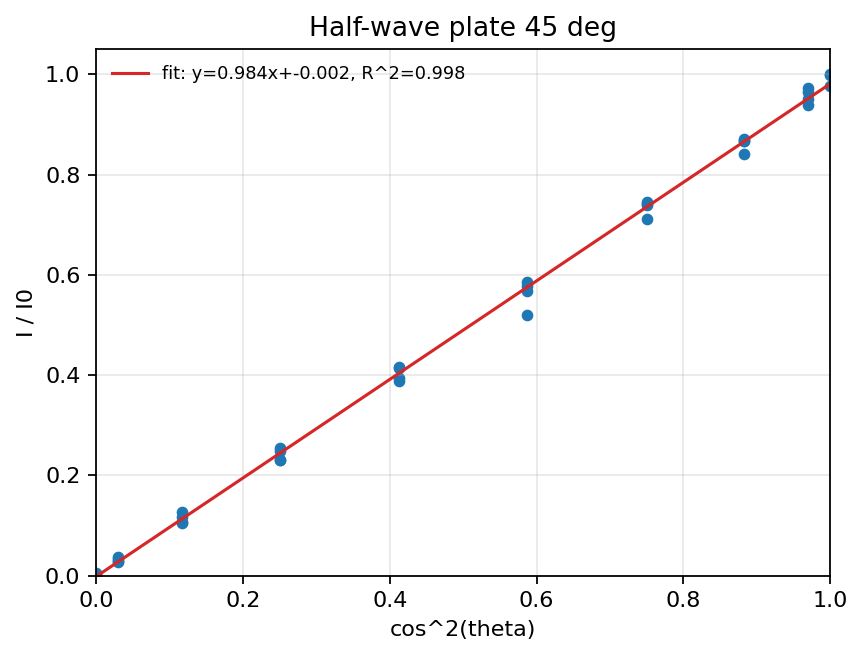
\includegraphics[width=\textwidth]{plots/half_cos2_45.png}\caption{$45^{\circ}$}\end{subfigure}
  \caption{$1/2$ 波片下 $I/I_0$ 与 $\cos^2\theta$ 的关系图}
  \label{fig:half-cos2}
\end{figure}

图\ref{fig:quarter-main} 与图\ref{fig:half-main} 分别给出了 $1/4$ 波片和 $1/2$ 波片的主实验曲线。可以直接看出，$1/4$ 波片在 $45^{\circ}$ 时的极坐标图最接近圆形，而 $1/2$ 波片的三条直角坐标曲线主要体现为峰位平移。图\ref{fig:quarter-cos2} 与图\ref{fig:half-cos2} 则用于辅助判断马吕斯定律是否仍可直接适用：当数据与 $\cos^2\theta$ 呈高线性相关时，说明出射光仍保持与参考零位一致的线偏振形式；当曲线明显偏离时，则意味着偏振态已经改变或偏振方向发生了整体旋转。

\section{实验结果与分析}
\subsection{$1/4$ 波片对偏振态的调制}
由图\ref{fig:quarter-main} 可见，当波片角度取 $0^{\circ}$ 时，直角坐标曲线呈典型双峰结构，极坐标图为标准双叶形，且 $I/I_0$ 与 $\cos^2\theta$ 的线性拟合相关系数达到 $R^2=0.995$。这说明此时出射光仍为线偏振光，$1/4$ 波片没有改变偏振类型，只引入了与单一主轴一致的传播过程。

当波片角度取 $30^{\circ}$ 时，透射光强的最小值仍有约 $0.200I_0$，最大值约为 $0.645I_0$，曲线起伏明显但始终不能消光，极坐标图表现为明显偏离圆形的闭合曲线。这说明两正交分量幅值不等且存在相位差，出射光应判定为椭圆偏振光。其与 $\cos^2\theta$ 的线性关系显著变差，$R^2$ 仅为 $0.315$，也说明马吕斯定律已不能直接描述该状态。

当波片角度取 $45^{\circ}$ 时，透射光强基本稳定在 $0.397I_0$ 到 $0.470I_0$ 之间，极坐标图接近圆形，说明检偏器旋转时透射光强近似不变，出射光为近似圆偏振光。曲线仍存在轻微起伏，表明实验所得并非理想圆偏振光，原因主要来自波片相位延迟的加工误差、零位标定偏差以及功率计读数波动。

\subsection{$1/2$ 波片对线偏振方向的旋转}
图\ref{fig:half-main} 显示，插入 $1/2$ 波片后，三组主实验曲线都保持了可消光的周期性变化，这说明出射光仍然是线偏振光。对于 $0^{\circ}$ 数据，峰值出现在约 $90^{\circ}$，最低点位于 $0^{\circ}$ 与 $180^{\circ}$ 附近，且与 $\cos^2\theta$ 的线性相关系数达到 $R^2=0.999$，完全符合参考零位下的马吕斯定律。

当 $1/2$ 波片转到 $30^{\circ}$ 时，曲线峰值移动到约 $150^{\circ}$，相较于 $0^{\circ}$ 数据平移了约 $60^{\circ}$；当波片转到 $45^{\circ}$ 时，峰值移动到 $0^{\circ}$ 或 $360^{\circ}$，对应平移约 $90^{\circ}$。这与理论上“线偏振光经过 $1/2$ 波片后振动方向旋转 $2\alpha$”完全一致：$2\times30^{\circ}=60^{\circ}$，$2\times45^{\circ}=90^{\circ}$。

图\ref{fig:half-cos2} 进一步给出了这一结论的细化解释。对 $0^{\circ}$ 和 $45^{\circ}$ 两组数据，$I/I_0$ 与 $\cos^2\theta$ 关系分别对应正斜率和负斜率直线，其中 $45^{\circ}$ 数据的拟合相关系数仍高达 $R^2=0.998$，说明其本质上相当于把原来的 $\cos^2\theta$ 曲线平移了 $90^{\circ}$，也即转化为 $\sin^2\theta$。而 $30^{\circ}$ 数据因对应相移为 $60^{\circ}$，相对于未修正的 $\cos^2\theta$ 不再保持线性，所以其 $R^2$ 下降到 $0.218$。这从另一个角度验证了 $1/2$ 波片不改变偏振类型，只改变偏振方向。

\section{误差分析}
本实验的主要误差首先来自角度零位的标定。起偏器、检偏器和波片均安装在独立卡架上，机械装配误差会使刻度盘读数与真实光轴方向之间存在固定偏差，因此必须依靠重新消光的方法确定 $\theta_1$、$\varphi_0$ 和 $\varphi_0'$。若零位判断略有偏差，曲线峰位就会整体平移，特别是对 $1/2$ 波片实验中的“转角翻倍”判据影响较大。

第二类误差来自波片本身的相位延迟与理想值不完全一致。实际 $1/4$ 波片未必恰好提供严格的 $\pi/2$ 相位差，因此在 $45^{\circ}$ 条件下得到的圆偏振光往往只是近似圆偏振光，从而表现为曲线仍有小幅起伏。第三类误差来自光源输出与功率计读数波动，特别是在低光强区间，读数抖动会相对放大，使最小值附近的散点偏离理想曲线。最后，记录单中未单独写明 $I_0$ 数值，因此本文取全部测量中的最大值 $10.04\,\mathrm{mW}$ 作为归一化基准，这会使部分曲线的峰值略低于 $1$，但不影响偏振态判别和峰位移动量分析。

\section{实验结论}
本实验利用真实记录单数据系统验证了偏振片与波片的基本作用规律。首先，起偏器和检偏器共同满足马吕斯定律，线偏振光在参考零位下可被检偏器完全消光。其次，$1/4$ 波片确实能够改变偏振态：当光轴与入射偏振方向夹角为 $0^{\circ}$ 时，出射光仍为线偏振光；为 $30^{\circ}$ 时，出射光变为椭圆偏振光；为 $45^{\circ}$ 时，出射光表现为近似圆偏振光。再次，$1/2$ 波片在保持线偏振属性的同时会使振动方向发生两倍角旋转，实验中 $30^{\circ}$ 和 $45^{\circ}$ 两组数据分别给出了约 $60^{\circ}$ 和 $90^{\circ}$ 的峰位平移，与理论完全一致。

\section{思考题}
\subsection*{思考题 1：怎样区分圆偏振光和线偏振光？}
线偏振光通过检偏器时会出现明显的极大值和极小值，并可在某一方向上完全消光；圆偏振光通过检偏器时透射光强与检偏器方位无关，旋转一周几乎保持常数。若担心圆偏振光与自然光混淆，可以在检偏器前加入 $1/4$ 波片：圆偏振光经过 $1/4$ 波片后会变成线偏振光，从而重新出现消光；线偏振光则在不满足特定角度条件时不会表现出这一特征。

\subsection*{思考题 2：怎样区分部分偏振光与椭圆偏振光？}
部分偏振光和椭圆偏振光都可能表现为“旋转检偏器时光强变化但不能消光”。区分方法是将 $1/4$ 波片的光轴与光强极大或极小方向对准，再继续旋转检偏器。若入射光为椭圆偏振光，则经过合适取向的 $1/4$ 波片后可转化为线偏振光，从而重新出现消光；若入射光为部分偏振光，则其非完全偏振成分不会被完全校正，仍然无法消光。

\subsection*{思考题 3：偏振片是否可以看作是光栅？为什么？}
一般不能把常见偏振片简单看作普通光栅。普通偏振片的主要机理是各向异性吸收或双折射，只允许某一振动方向的电场分量通过，并不是依靠多缝衍射或路径差干涉来工作。只有金属丝栅偏振器这类具有亚波长周期结构的器件，才在一定意义上兼具“栅状结构”和偏振选择功能，但其工作本质仍然是对不同偏振分量的电磁响应差异，而不是通常意义上的衍射光栅成像机制。

\appendix
\renewcommand{\thefigure}{\Alph{section}-\arabic{figure}}
\renewcommand{\thetable}{\Alph{section}-\arabic{table}}

\section{原始数据记录}
根据实验要求，完整的真实数据记录单及签字页附于本报告末尾。图\ref{fig:raw-1} 至图\ref{fig:raw-4} 保留了记录单原貌，其中第 1 页和第 3 页包含手写原始数据与教师签字，第 2 页和第 4 页保留了原始绘图区版式。

\begin{figure}[H]
  \centering
  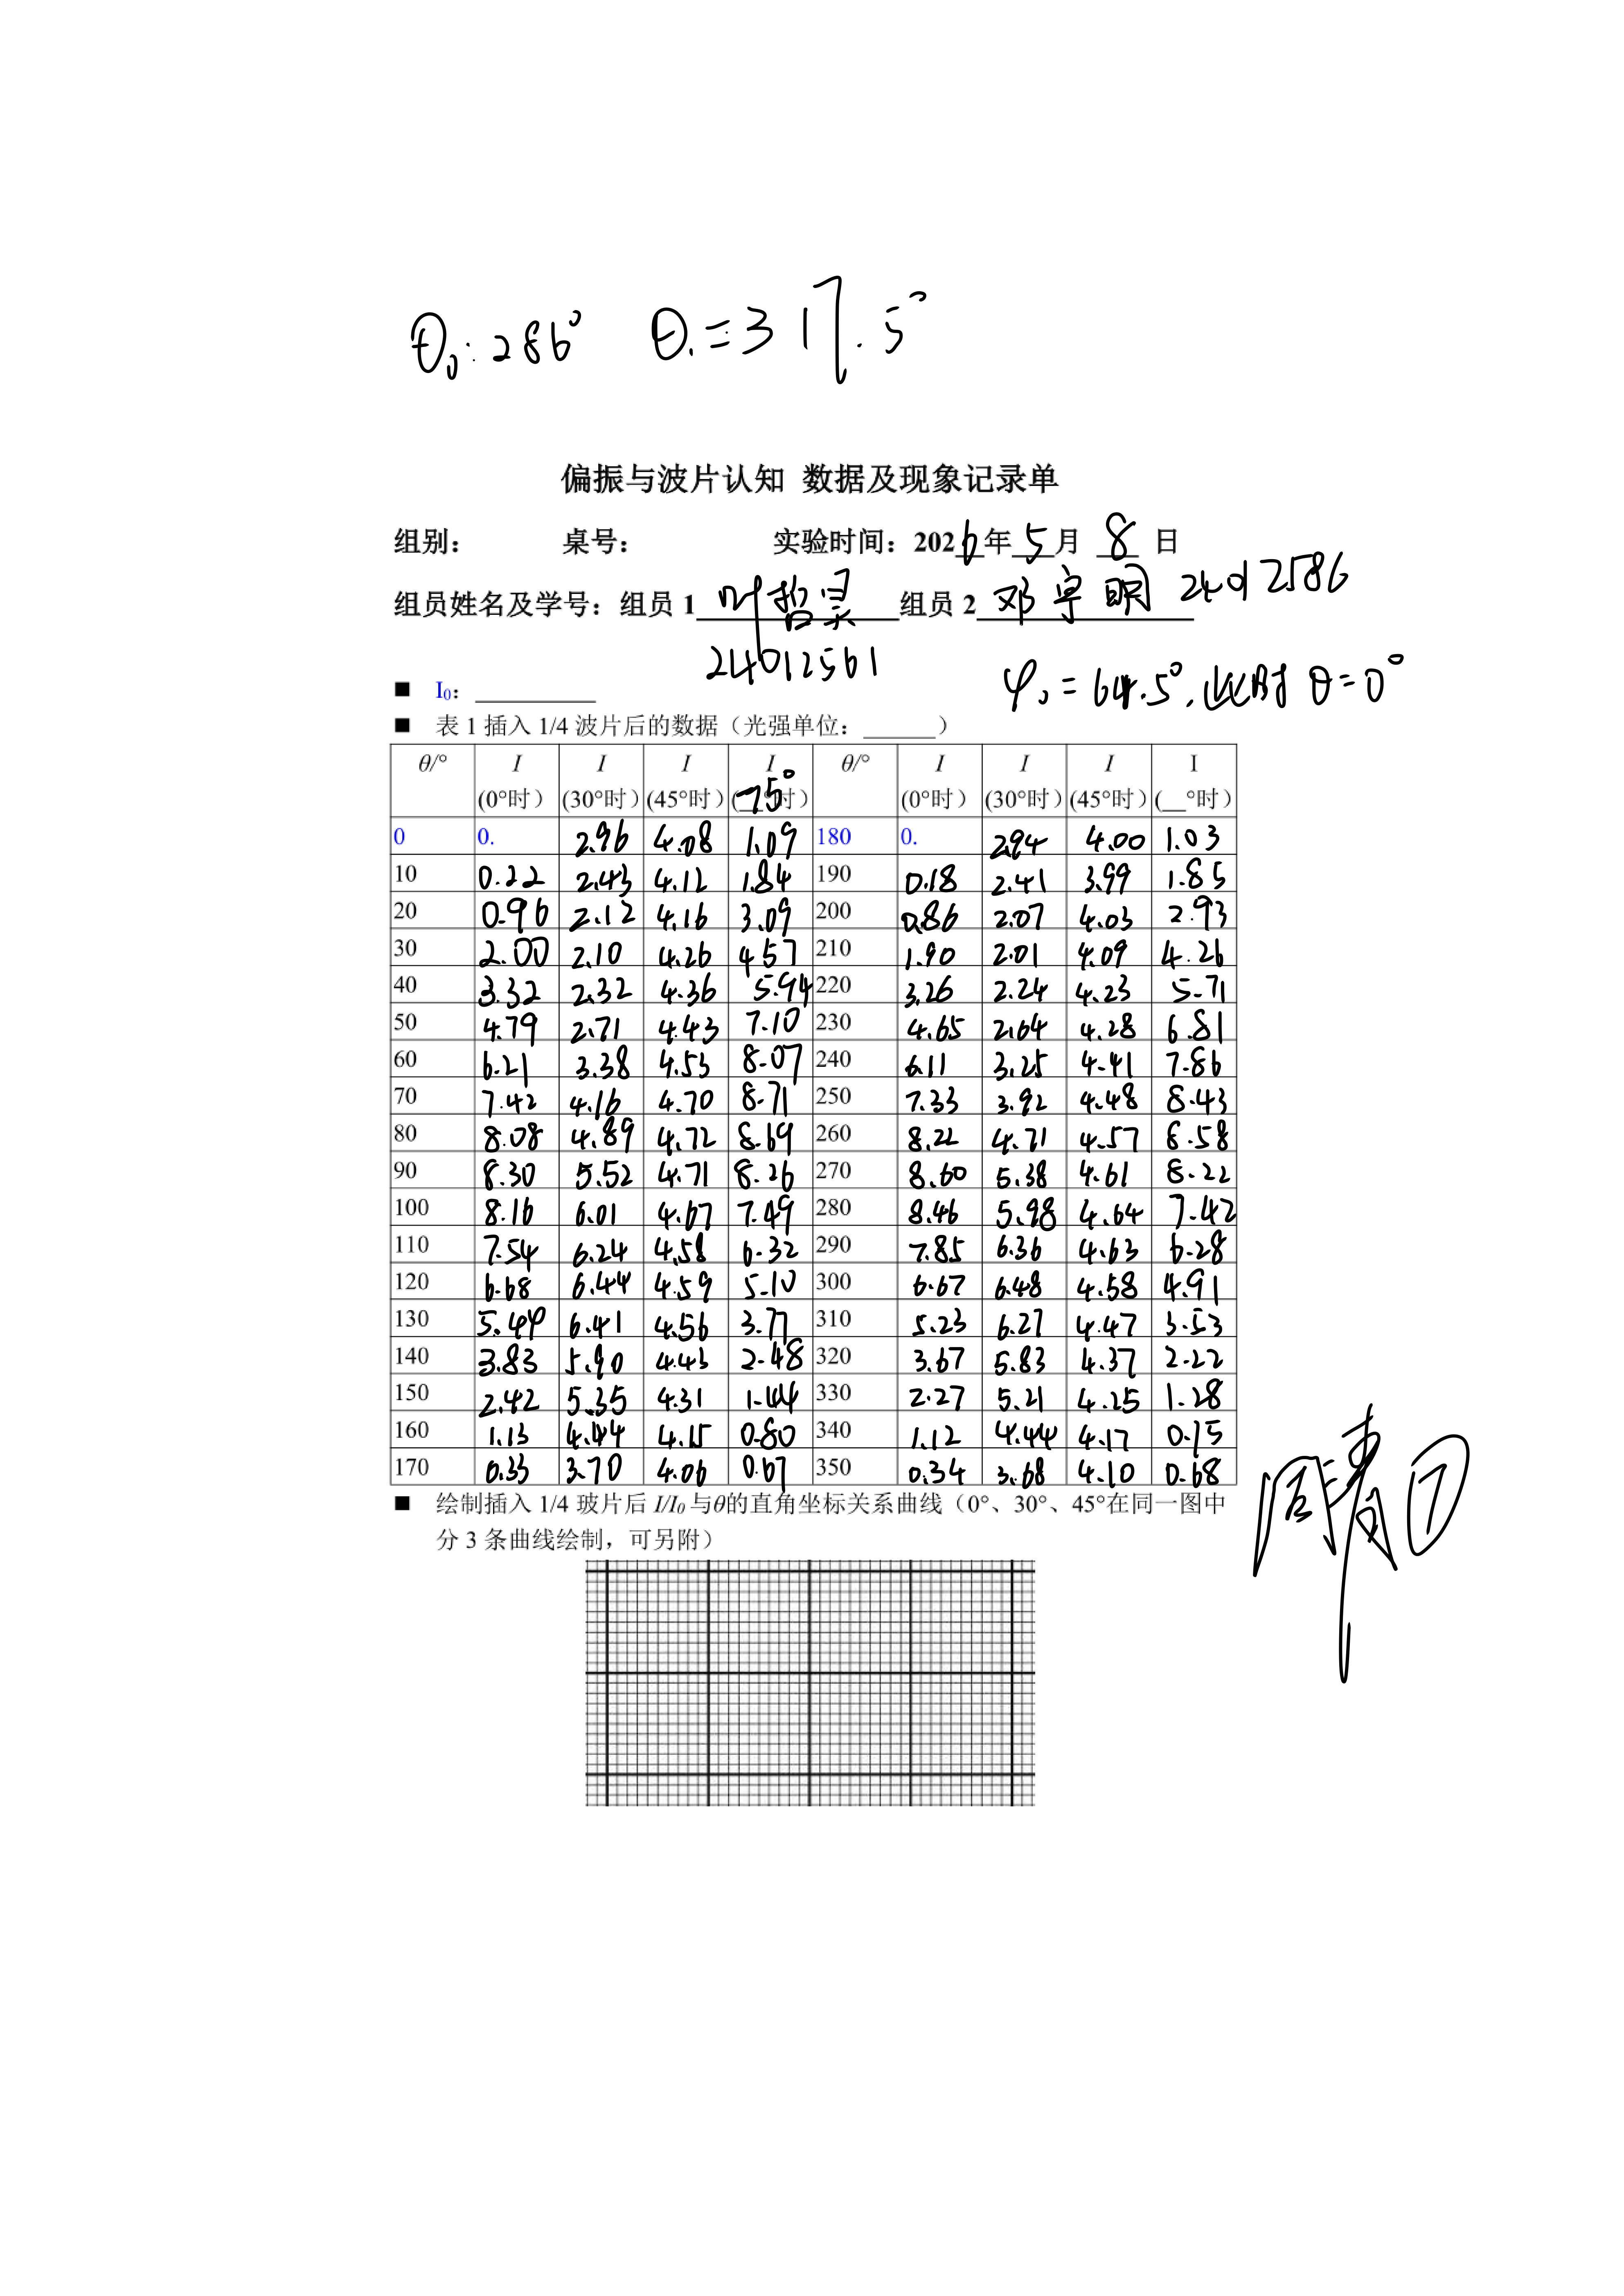
\includegraphics[width=0.82\textwidth]{偏振与波片认识实验数据记录单/偏振与波片认识实验数据记录单_01.png}
  \caption{原始数据记录单第 1 页：实验信息与 $1/4$ 波片原始数据}
  \label{fig:raw-1}
\end{figure}

\begin{figure}[H]
  \centering
  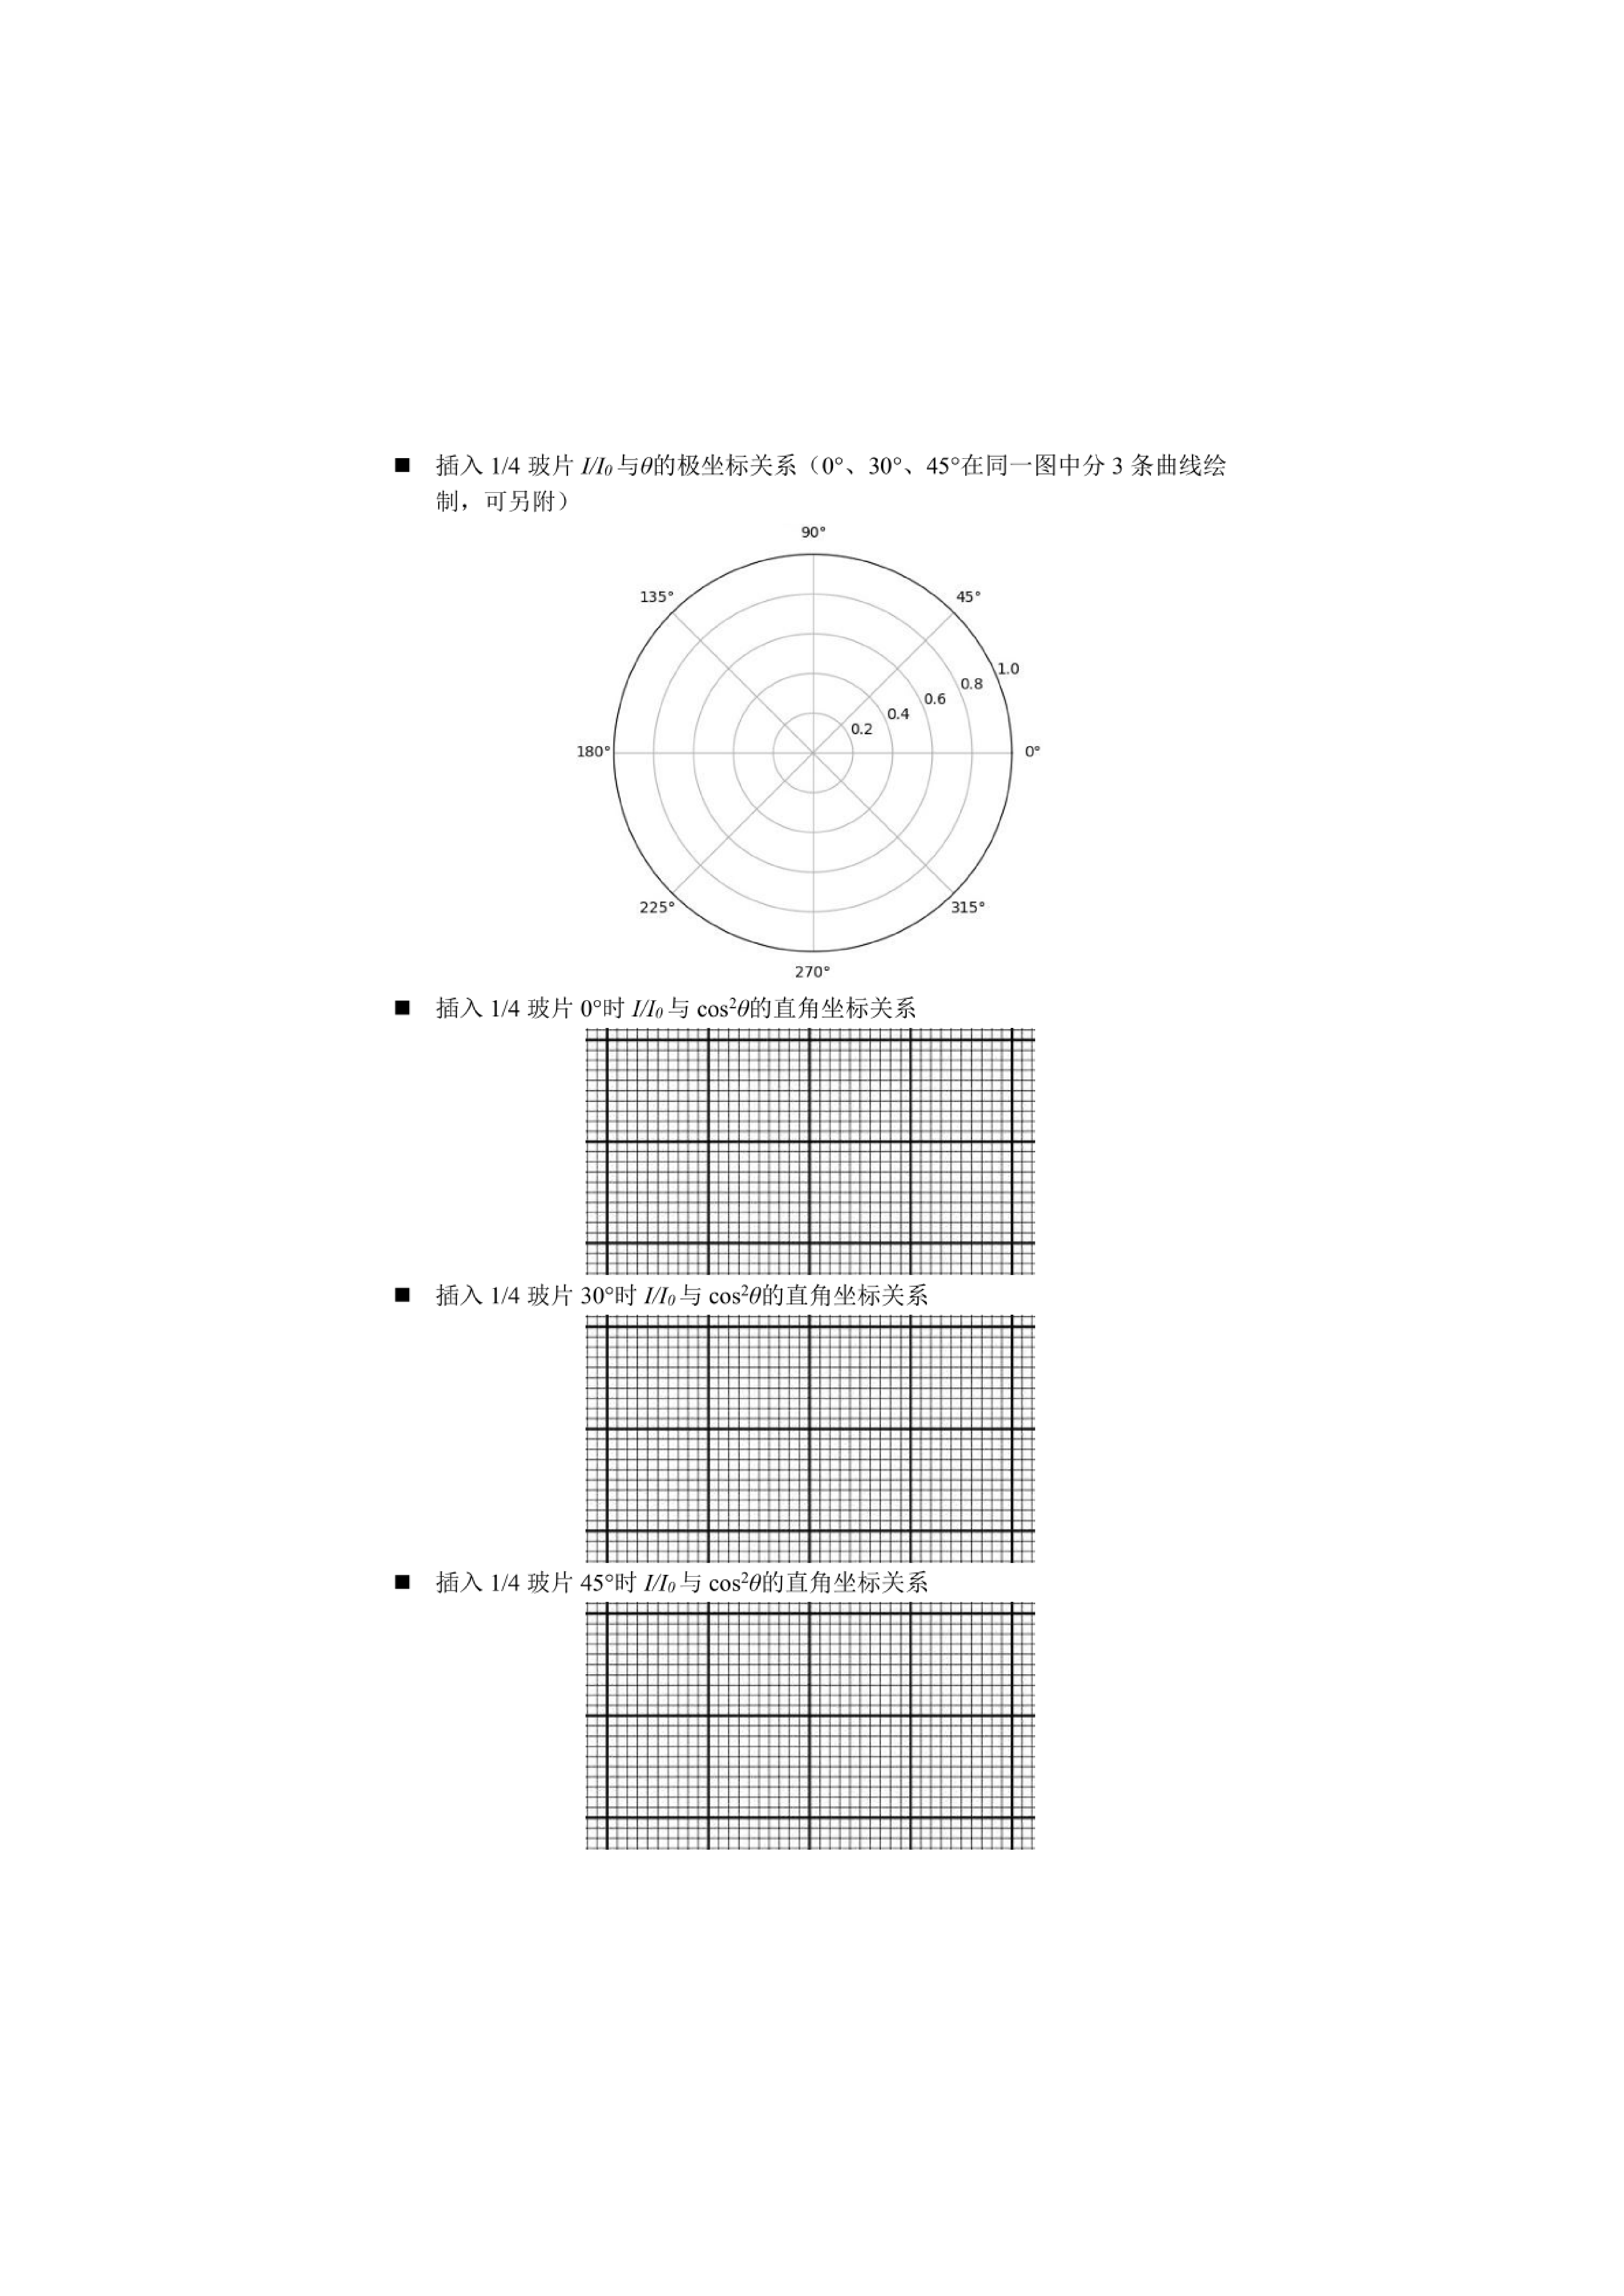
\includegraphics[width=0.82\textwidth]{偏振与波片认识实验数据记录单/偏振与波片认识实验数据记录单_02.png}
  \caption{原始数据记录单第 2 页：$1/4$ 波片绘图区}
  \label{fig:raw-2}
\end{figure}

\begin{figure}[H]
  \centering
  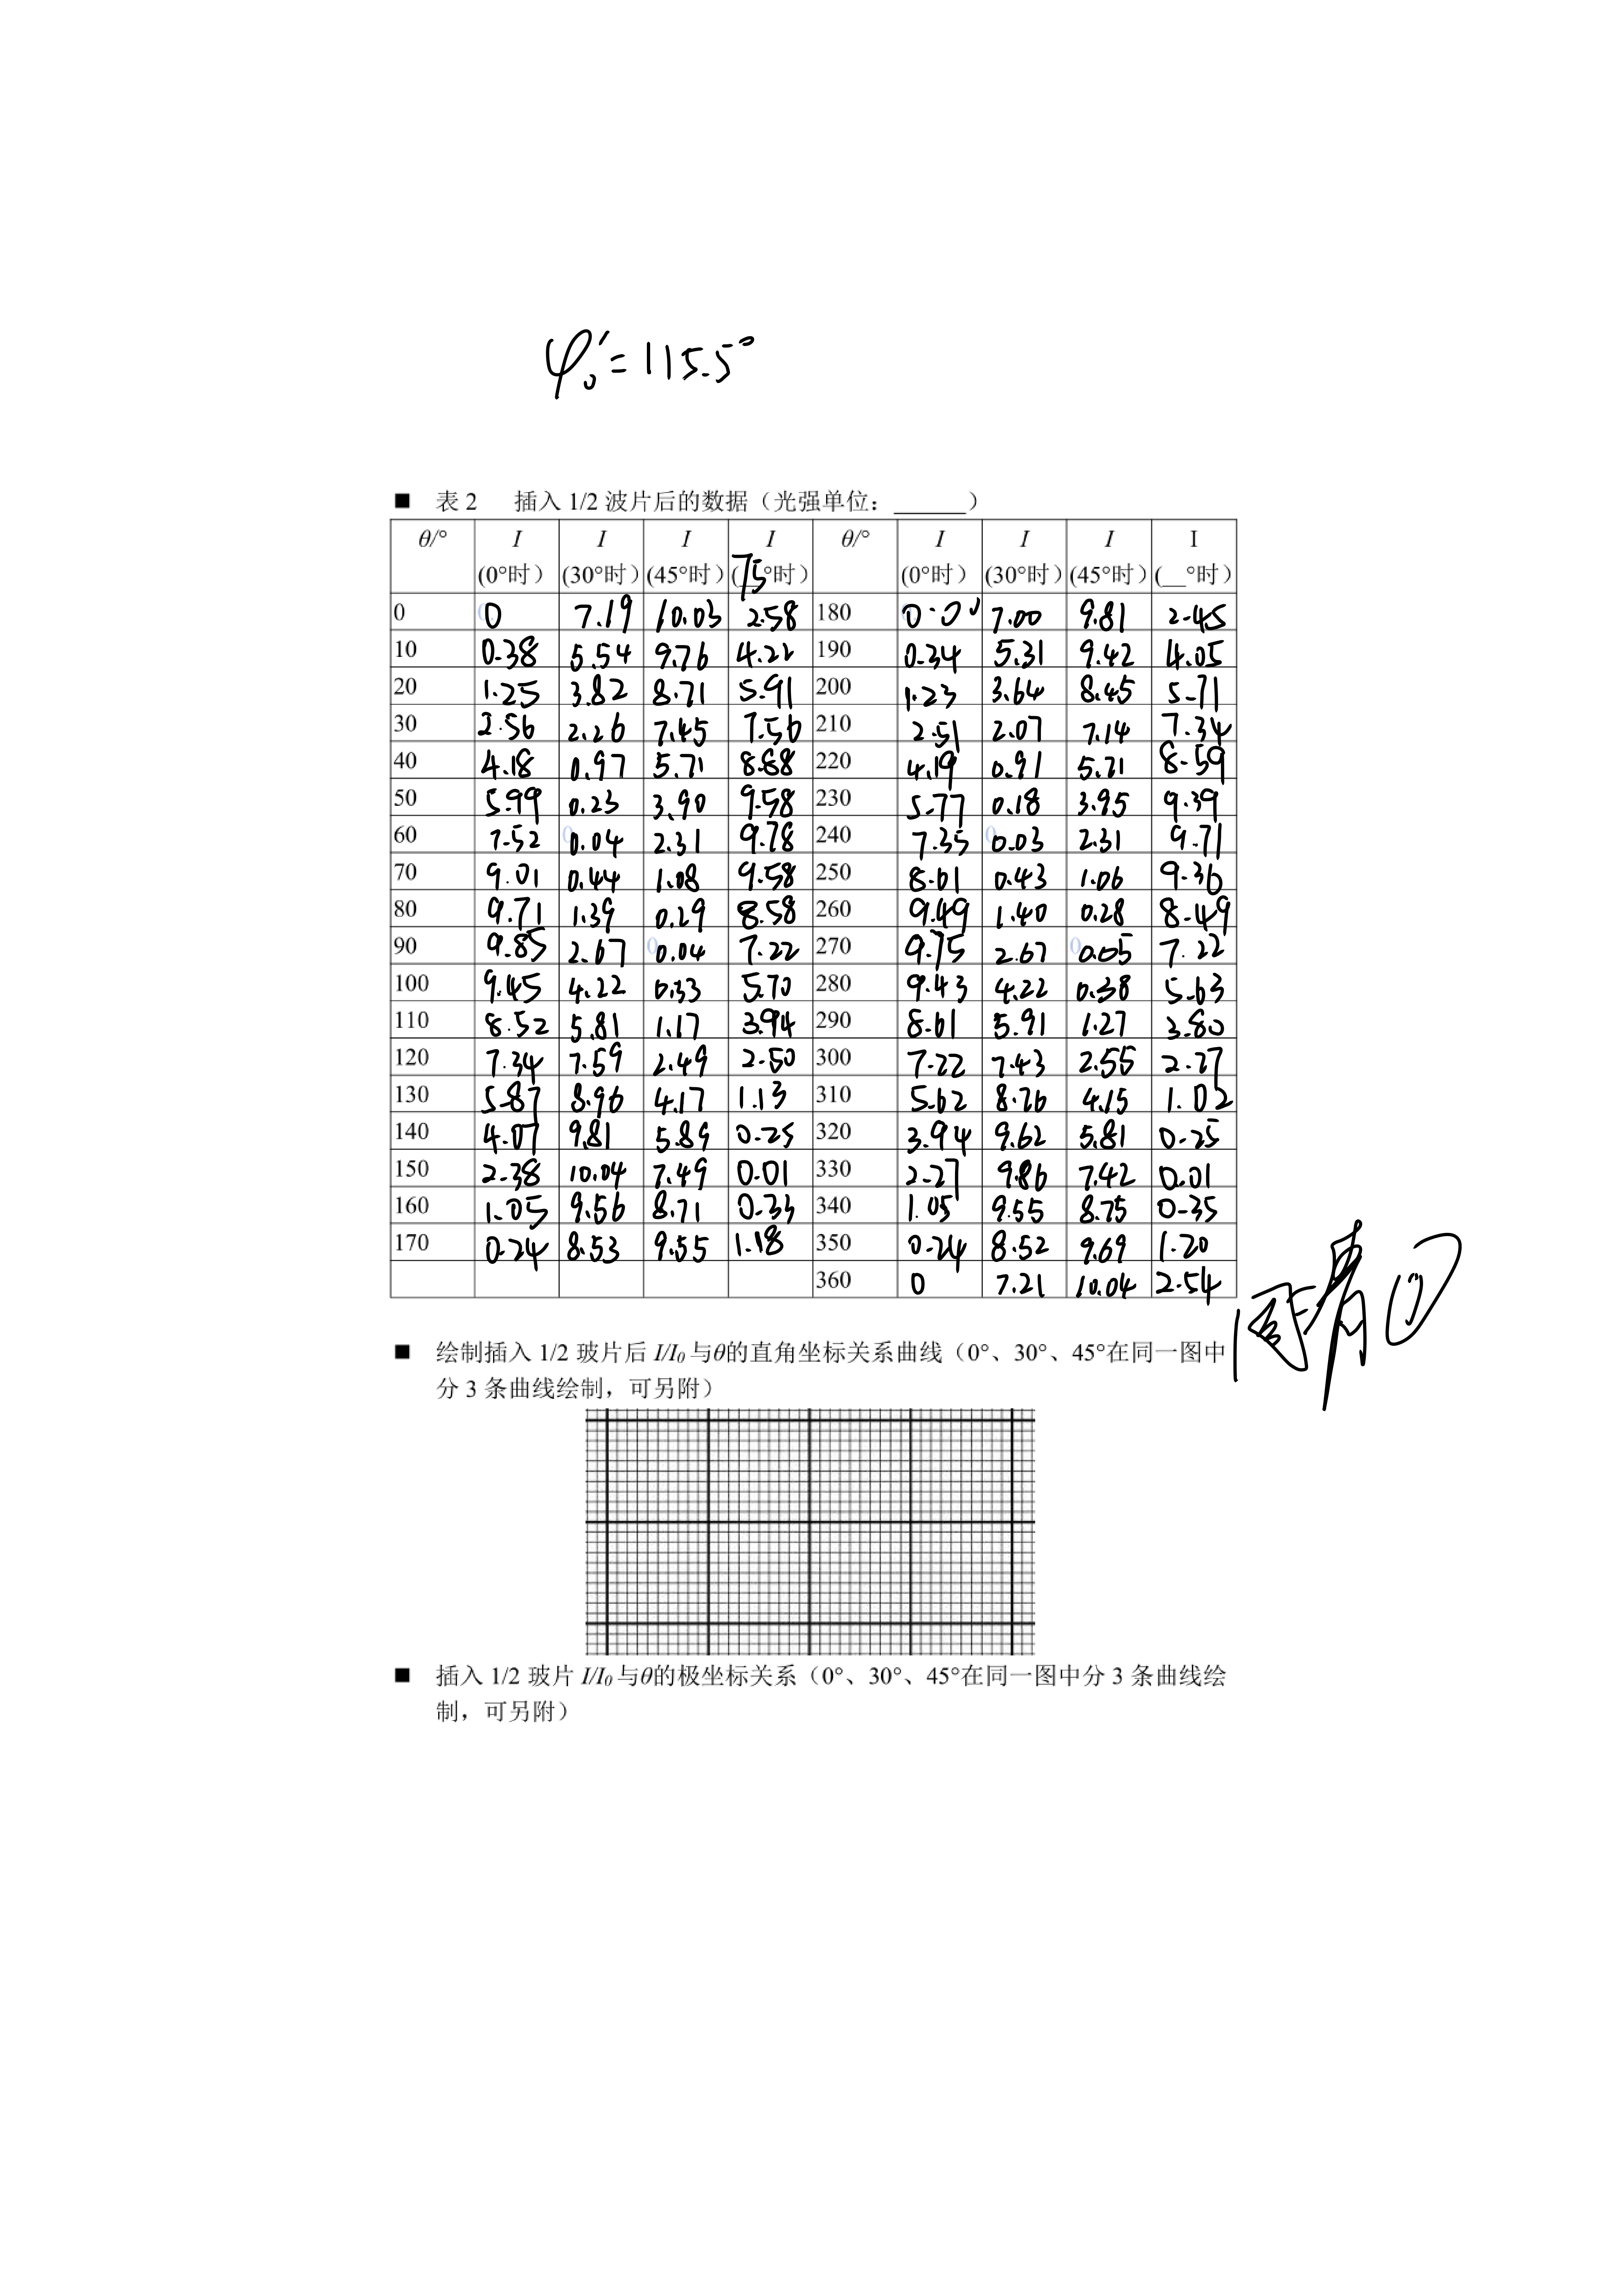
\includegraphics[width=0.82\textwidth]{偏振与波片认识实验数据记录单/偏振与波片认识实验数据记录单_03.png}
  \caption{原始数据记录单第 3 页：$1/2$ 波片原始数据}
  \label{fig:raw-3}
\end{figure}

\begin{figure}[H]
  \centering
  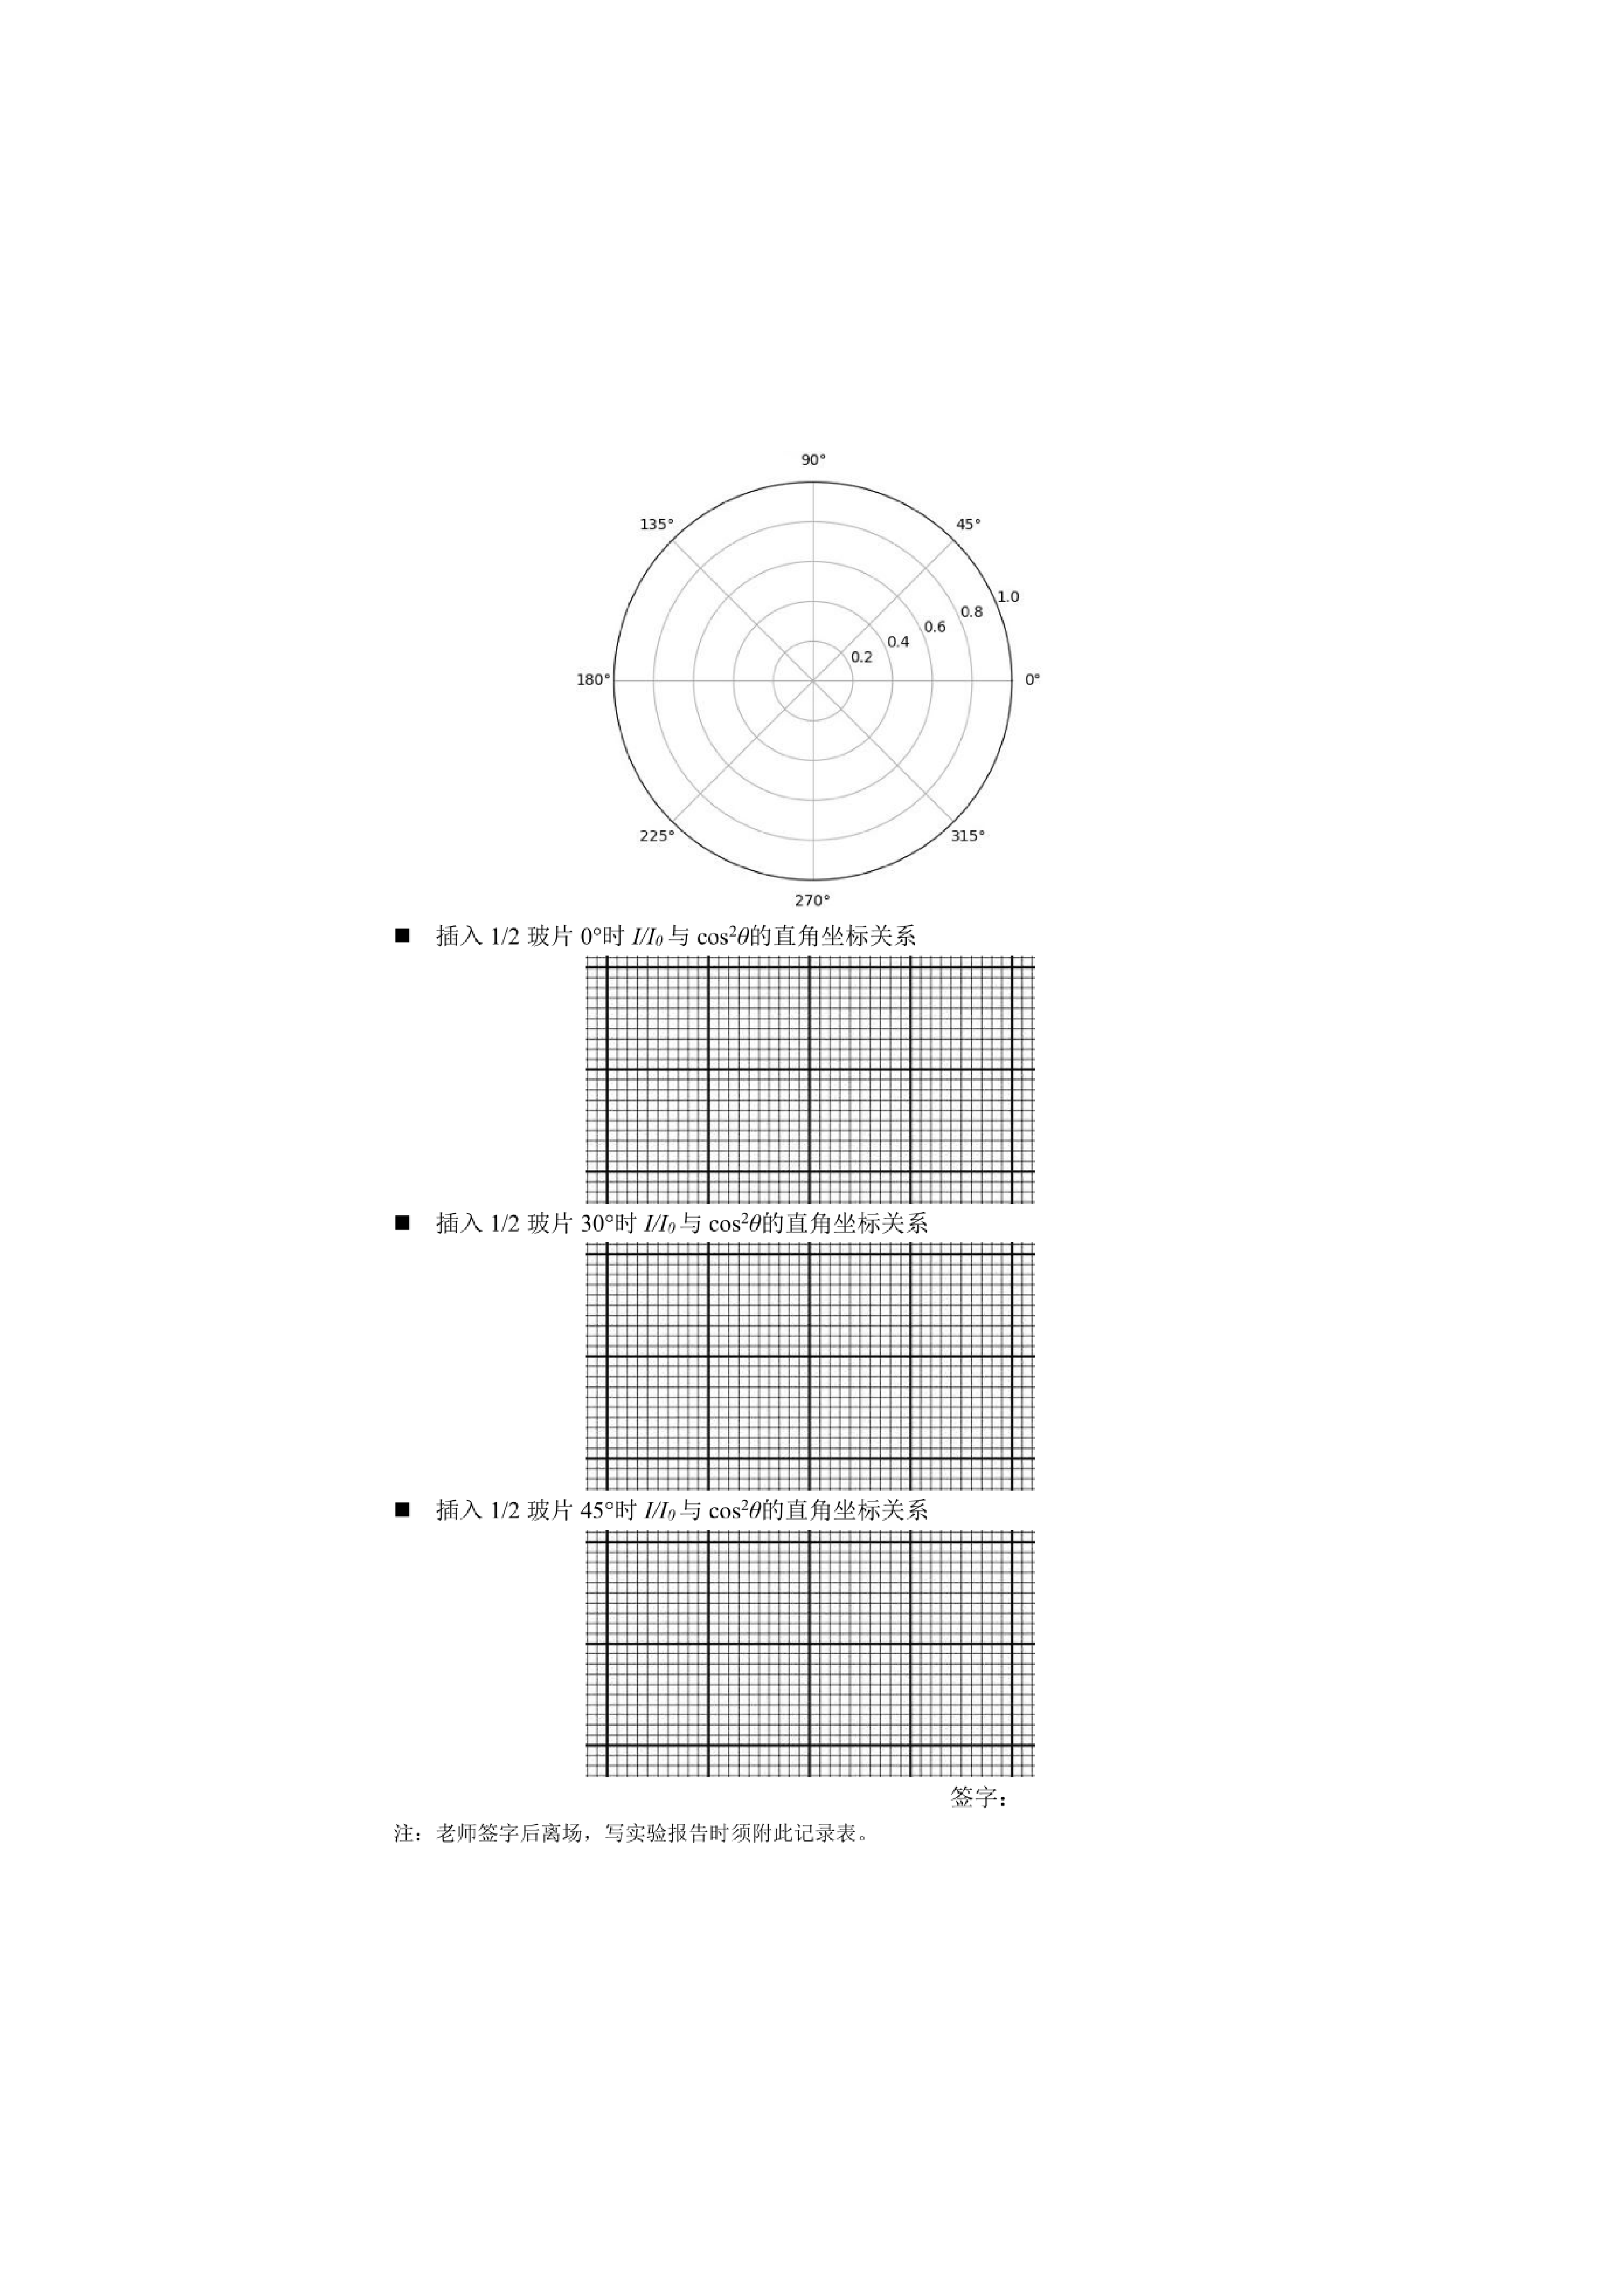
\includegraphics[width=0.82\textwidth]{偏振与波片认识实验数据记录单/偏振与波片认识实验数据记录单_04.png}
  \caption{原始数据记录单第 4 页：$1/2$ 波片绘图区与签字区}
  \label{fig:raw-4}
\end{figure}

\end{document}